\documentclass[a4paper,12pt,twoside]{book}
\usepackage{textfit}
\usepackage{phdthesis}
\usepackage{titlepage_moa}
\usepackage{amsthm}
\usepackage[bitstream-charter]{mathdesign}
%
\usepackage{listings}
\usepackage{graphicx}
\usepackage{epstopdf}
\usepackage{tikz} 
\usepackage{hyperref}
\usepackage{algorithm,algorithmic}
\definecolor{nicered}{rgb}{0.0,0.0,0.4}

\hypersetup{
    bookmarks=true,         % show bookmarks bar?
    unicode=false,          % non-Latin characters in Acrobat’s bookmarks
    pdftoolbar=true,        % show Acrobat’s toolbar?
    pdfmenubar=true,        % show Acrobat’s menu?
    pdffitwindow=false,     % window fit to page when opened
    pdfstartview={FitV},    % fits the width of the page to the window
    pdftitle={MOA Manual},    % title
    pdfauthor={Albert Bifet, Richard Kirkby, Philipp Kranen, Peter Reutemann},     % author
    pdfsubject={},   % subject of the document
    pdfcreator={Albert Bifet, Richard Kirkby, Philipp Kranen, Peter Reutemann},   % creator of the document
    pdfproducer={Albert Bifet, Richard Kirkby, Philipp Kranen, Peter Reutemann}, % producer of the document
    pdfkeywords={}, % list of keywords
    pdfnewwindow=true,      % links in new window
    colorlinks=true,       % false: boxed links; true: colored links
    linkcolor=nicered,          % color of internal links
    citecolor=blue,        % color of links to bibliography
    filecolor=magenta,      % color of file links
    urlcolor=cyan           % color of external links
}

\long\def\BEGINOMIT#1\ENDOMIT{\relax}  % to omit large portions of text
\newtheorem{definition}{Definition}{}
\title{
\textbf{Massive Online Analysis}  \\ 
Manual
}
\author{Albert Bifet, Richard Kirkby, \\Philipp Kranen, Peter Reutemann }
\date{March 2012}
\begin{document}
\lstset{language=Java,basicstyle=\tiny,numbers=left}

\pdfbookmark[0]{Titlepage}{title} 
\maketitle
\pagenumbering{roman}
\thispagestyle{empty}
\cleardoublepage
%\ENDOMIT
\thispagestyle{empty}
%\setcounter{page}{1}
\pdfbookmark[0]{Contents}{contents}
\tableofcontents
\cleardoublepage
%\listoffigures
%\listoftables
\pagenumbering{arabic}

\chapter{Introduction}

{\bf M}assive {\bf O}nline {\bf A}nalysis (MOA) 
is a software environment for implementing algorithms and running experiments for online learning from evolving data streams. 
MOA is designed to deal with the challenging problems of scaling up the implementation of state of the art algorithms to real 
world dataset sizes and of making algorithms comparable in benchmark streaming settings.

\begin{center}

\includegraphics[height=2cm]{images/LogoMOA.jpg} \end{center}

MOA contains a collection of offline 
and online algorithms for both classification and clustering as well as tools for evaluation.  
Researchers benefit from MOA by getting insights into workings and problems of different approaches, practitioners can 
easily compare several algorithms and apply them to real world data sets and settings. 

MOA supports bi-directional interaction
 with WEKA, the Waikato Environment for Knowledge Analysis, 
which is an award-winning open-source 
workbench containing implementations of a wide range of batch machine 
learning methods. WEKA is also written in Java. The main benefits
of Java are portability, where applications can be run on any platform with
an appropriate Java virtual machine, and the strong and well-developed support 
libraries. Use of the language is widespread, and features such as the
automatic garbage collection help to reduce programmer burden and error.

    One of the key data structures used in MOA is the description of an example
from a data stream. This structure borrows from WEKA, where an example is
represented by an array of double precision floating point values. This provides
freedom to store all necessary types of value \--- numeric attribute values can be
stored directly, and discrete attribute values and class labels are represented
by integer index values that are stored as floating point values in the array.
Double precision floating point values require storage space of 64 bits, or 8
bytes. This detail can have implications for memory usage. %utilization.

\section{Data streams Evaluation}
A data stream environment has different requirements from the traditional 
setting. The most significant are the following: 
\begin{description}
\item[Requirement 1] Process an example at a time, and inspect
 it only once (at most)
\item[Requirement 2] Use a limited amount of memory
\item[Requirement 3] Work in a limited amount of time
\item[Requirement 4] Be ready to predict at any time
\end{description}
\begin{figure}[t]
\begin{center} 
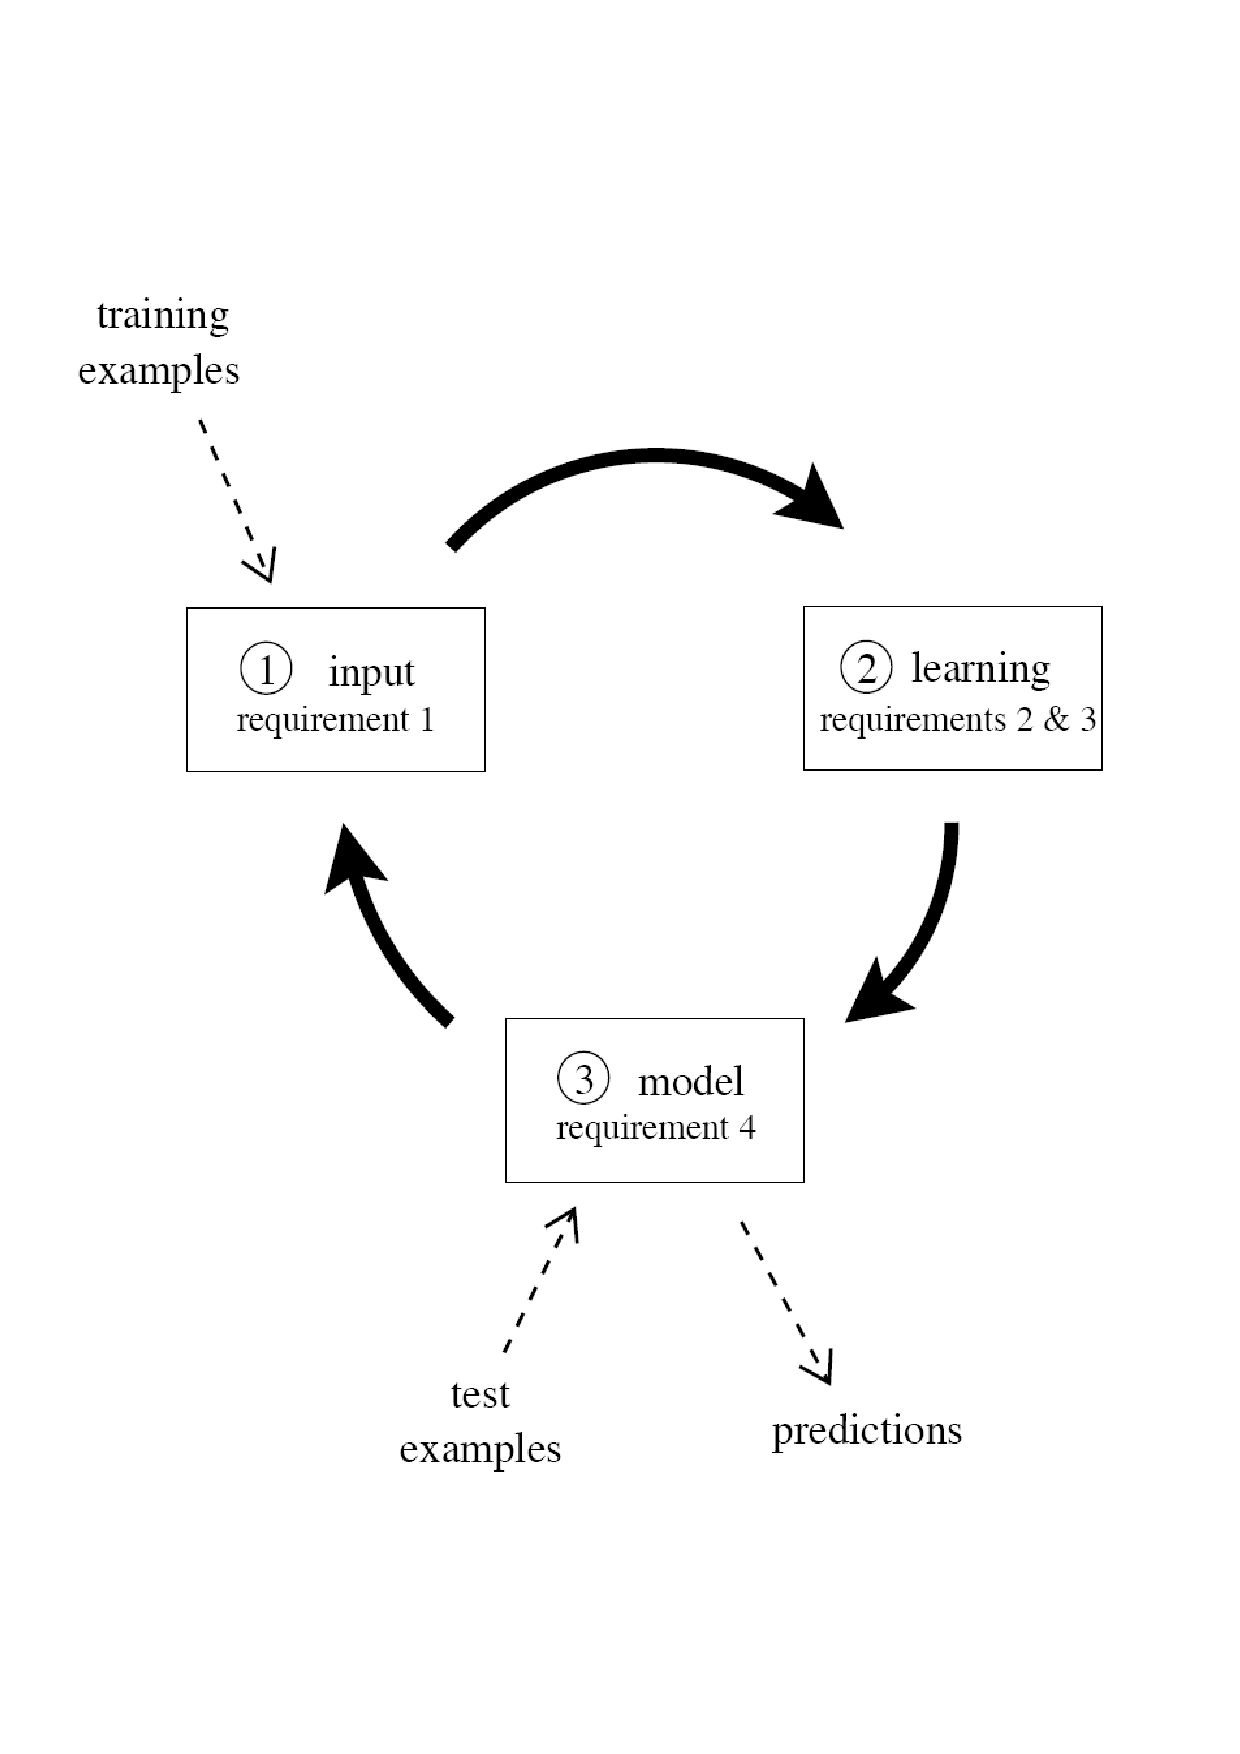
\includegraphics[height=9cm]{images/Frame.pdf}
\end{center} 
\caption{The data stream classification cycle}
\label{fig:cycle}
\end{figure} 
We have to consider these requirements in order to design a new experimental
framework for data streams.
Figure~\ref{fig:cycle} illustrates the typical use of a data stream 
classification algorithm, and how the requirements fit
in a repeating cycle:
\begin{enumerate}
\item  The algorithm is passed the next available example from the stream
   (requirement 1).
\item  The algorithm processes the example, updating its data structures. It
   does so without exceeding the memory bounds set on it (requirement 2),
   and as quickly as possible (requirement 3).
\item  The algorithm is ready to accept the next example. On request it is
   able to predict the class of unseen examples
   (requirement 4).
\end{enumerate}
\BEGINOMIT
We define three environments that are simulated using memory limits, 
since memory limits cannot be ignored and can significantly limit capacity
to learn from data streams. Potential practical deployment of data stream
classification has been divided into scenarios of increasing memory utilization,
from the restrictive sensor environment, to a typical consumer grade handheld
PDA environment, to the least restrictive environment of a dedicated server.

\begin{description}
\item[Sensor Network] This environment represents the most restrictive case, 
learning in 100 kilobytes of memory. Because this limit is so restrictive,
it is an interesting test case for algorithm efficiency.

\item[Handheld Computer] In this case the algorithm is allowed 32 megabytes of 
memory. This simulates the capacity of lightweight consumer devices designed to
be carried around by users and fit into a shirt pocket.

\item[Server] This environment simulates either a modern laptop/desktop computer
or server dedicated to processing a data stream. The memory limit assigned in 
this environment is 400 megabytes.  Considering that several algorithms have 
difficulty in fully utilizing this much working space, it seems sufficiently 
realistic to impose this limit.

\end{description}
\ENDOMIT
In traditional batch learning the problem of limited data is overcome
by analyzing and averaging multiple models produced with different random
arrangements of training and test data. In the stream setting the problem of
(effectively) unlimited data poses different challenges. One solution involves
taking snapshots at different times during the induction of a model to see how
much the model improves.

The evaluation procedure of a learning algorithm determines which examples
are used for training the algorithm, and which are used to test the model output
by the algorithm. The procedure used historically in batch learning has partly
depended on data size. As data sizes increase, practical
time limitations prevent procedures that repeat training too many times. It is
commonly accepted with considerably larger data sources that it is necessary
to reduce the numbers of repetitions or folds to allow experiments to complete
in reasonable time. 
    When considering what procedure to use in the data stream setting, one of
the unique concerns is how to build a picture of accuracy over time. Two main
approaches arise:
\begin{itemize}
 \item {\bf Holdout}:
When traditional batch learning reaches a scale where cross-validation is too time 
consuming, it is often accepted to instead measure performance on a single holdout
set. This is most useful when the division between train and test sets have
been pre-defined, so that results from different studies can be directly compared. 
\item {\bf Interleaved Test-Then-Train or Prequential}:
 Each individual example can be used to test the model
before it is used for training, and from this the accuracy can be incrementally
updated. When intentionally performed in this order, the model is always
being tested on examples it has not seen. This scheme has the advantage that
no holdout set is needed for testing, making maximum use of the available
data. It also ensures a smooth plot of accuracy over time, as each individual
example will become increasingly less significant to the overall average.
\end{itemize}
   As data stream classification is a relatively new field, such evaluation 
practices are not nearly as well researched and established as they are
in the traditional batch setting. 
The majority of experimental evaluations use less than one million
training examples. 
In the context of data streams this is disappointing, because to be
truly useful at data stream classification the algorithms need to be capable of 
handling very large (potentially infinite) streams of examples. Demonstrating 
systems only on small amounts of data does not build a convincing case for capacity
to solve more demanding data stream applications.

    MOA permits adequately evaluate data stream
classification algorithms on large streams, in the order
of tens of millions of examples where possible, and under explicit memory
limits. Any less than this does not actually test algorithms in a realistically
challenging setting. 

\chapter{Installation}

The following manual is based on a Unix/Linux system with Java 6 SDK or greater installed. 
Other operating systems such as Microsoft Windows will be similar but may need adjustments to suit.

MOA needs the following files:

\begin{itemize}
\item \texttt{moa.jar}
\item \texttt{sizeofag.jar}
\end{itemize}
They are available from
\begin{itemize}
\item \texttt{http://sourceforge.net/projects/moa-datastream/}
\item \texttt{http://www.jroller.com/resources/m/maxim/sizeofag.jar}
\end{itemize}
These files are needed to run the MOA software from the command line:
\begin{verbatim}
java -Xmx4G -cp moa.jar -javaagent:sizeofag.jar moa.DoTask \
  LearnModel -l DecisionStump \
  -s generators.WaveformGenerator \
  -m 1000000 -O model1.moa
\end{verbatim}
 and the graphical interface:
\begin{verbatim}
java -Xmx4G -cp moa.jar -javaagent:sizeofag.jar moa.gui.GUI
\end{verbatim}

\texttt{Xmx4G} increases the maximum heap size to 4GB for your java engine, as
the default setting of 16 to 64MB may be too small. 


\section{WEKA}
\label{sec:InstWeka}

It is possible to use the classifiers available in WEKA 3.7. The file \texttt{weka.jar} is available from
\begin{verbatim}
http://sourceforge.net/projects/weka/files/weka-3-7/
\end{verbatim}

This file is needed to run the MOA software with WEKA from the command line:
\begin{verbatim}
java -Xmx4G -cp moa.jar:weka.jar -javaagent:sizeofag.jar 
  moa.DoTask "LearnModel \
  -l (WekaClassifier -l weka.classifiers.trees.J48) \ 
  -s generators.WaveformGenerator -m 1000000 -O model1.moa"
\end{verbatim}
and the graphical interface:
\begin{verbatim}
java -Xmx4G -cp moa.jar:weka.jar -javaagent:sizeofag.jar \
    moa.gui.GUI
\end{verbatim}
or, using Microsoft Windows:
\begin{verbatim}
java -Xmx4G -cp moa.jar;weka.jar -javaagent:sizeofag.jar
  moa.DoTask "LearnModel 
  -l (WekaClassifier -l weka.classifiers.trees.J48)                  
  -s generators.WaveformGenerator -m 1000000 -O model1.moa"

java -Xmx4G -cp moa.jar;weka.jar -javaagent:sizeofag.jar 
    moa.gui.GUI
\end{verbatim}


\chapter{Using MOA}
\section{Using the GUI}
A graphical user interface for configuring and running tasks is available with the command:

\begin{verbatim}
java -Xmx4G -cp moa.jar -javaagent:sizeofag.jar moa.gui.GUI
\end{verbatim}

There are two main tabs: one for classification and one for clustering.

\subsection{Classification}

\begin{figure}[ht]
\begin{center}
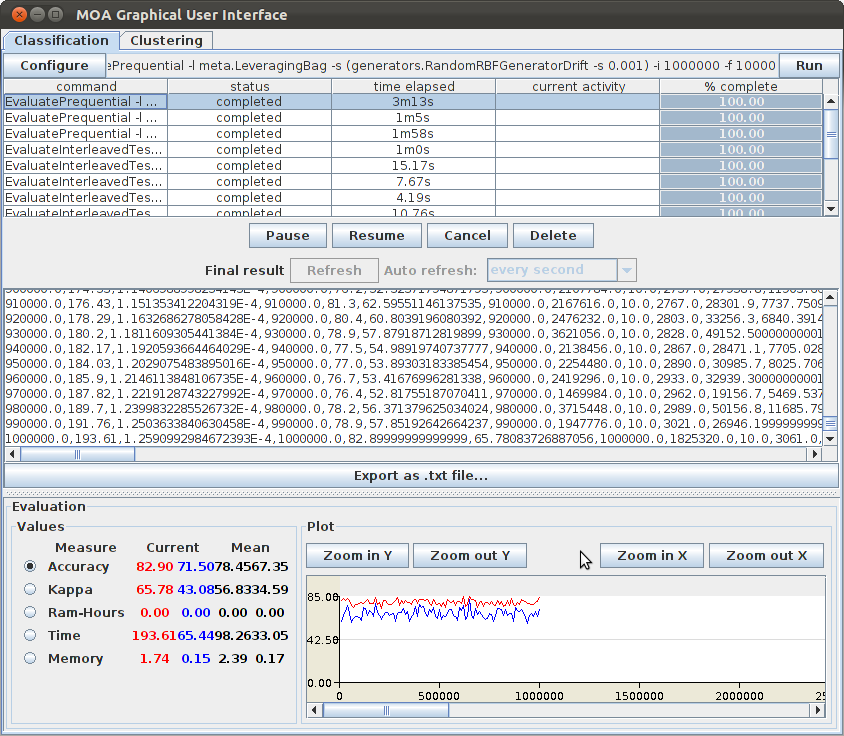
\includegraphics[height=6cm]{images/MOA_Task.png}\end{center}
\caption{Graphical user interface of MOA}
\end{figure}

Click 'Configure' to set up a task, when ready click to launch a task click 'Run'. Several tasks can be run concurrently. Click on different tasks in the list and control them using the buttons below. If textual output of a task is available it will be displayed in the bottom half of the GUI, and can be saved to disk.

Note that the command line text box displayed at the top of the window represents textual commands that can be used to run tasks on the command line as described in the next chapter.
The text can be selected then copied onto the clipboard. 
In the bottom of the GUI there is a graphical display of the results. It is possible
to compare the results of two different tasks: the current task is displayed in red, and the selected previously is in blue. 

\begin{figure}[t]
\begin{center}
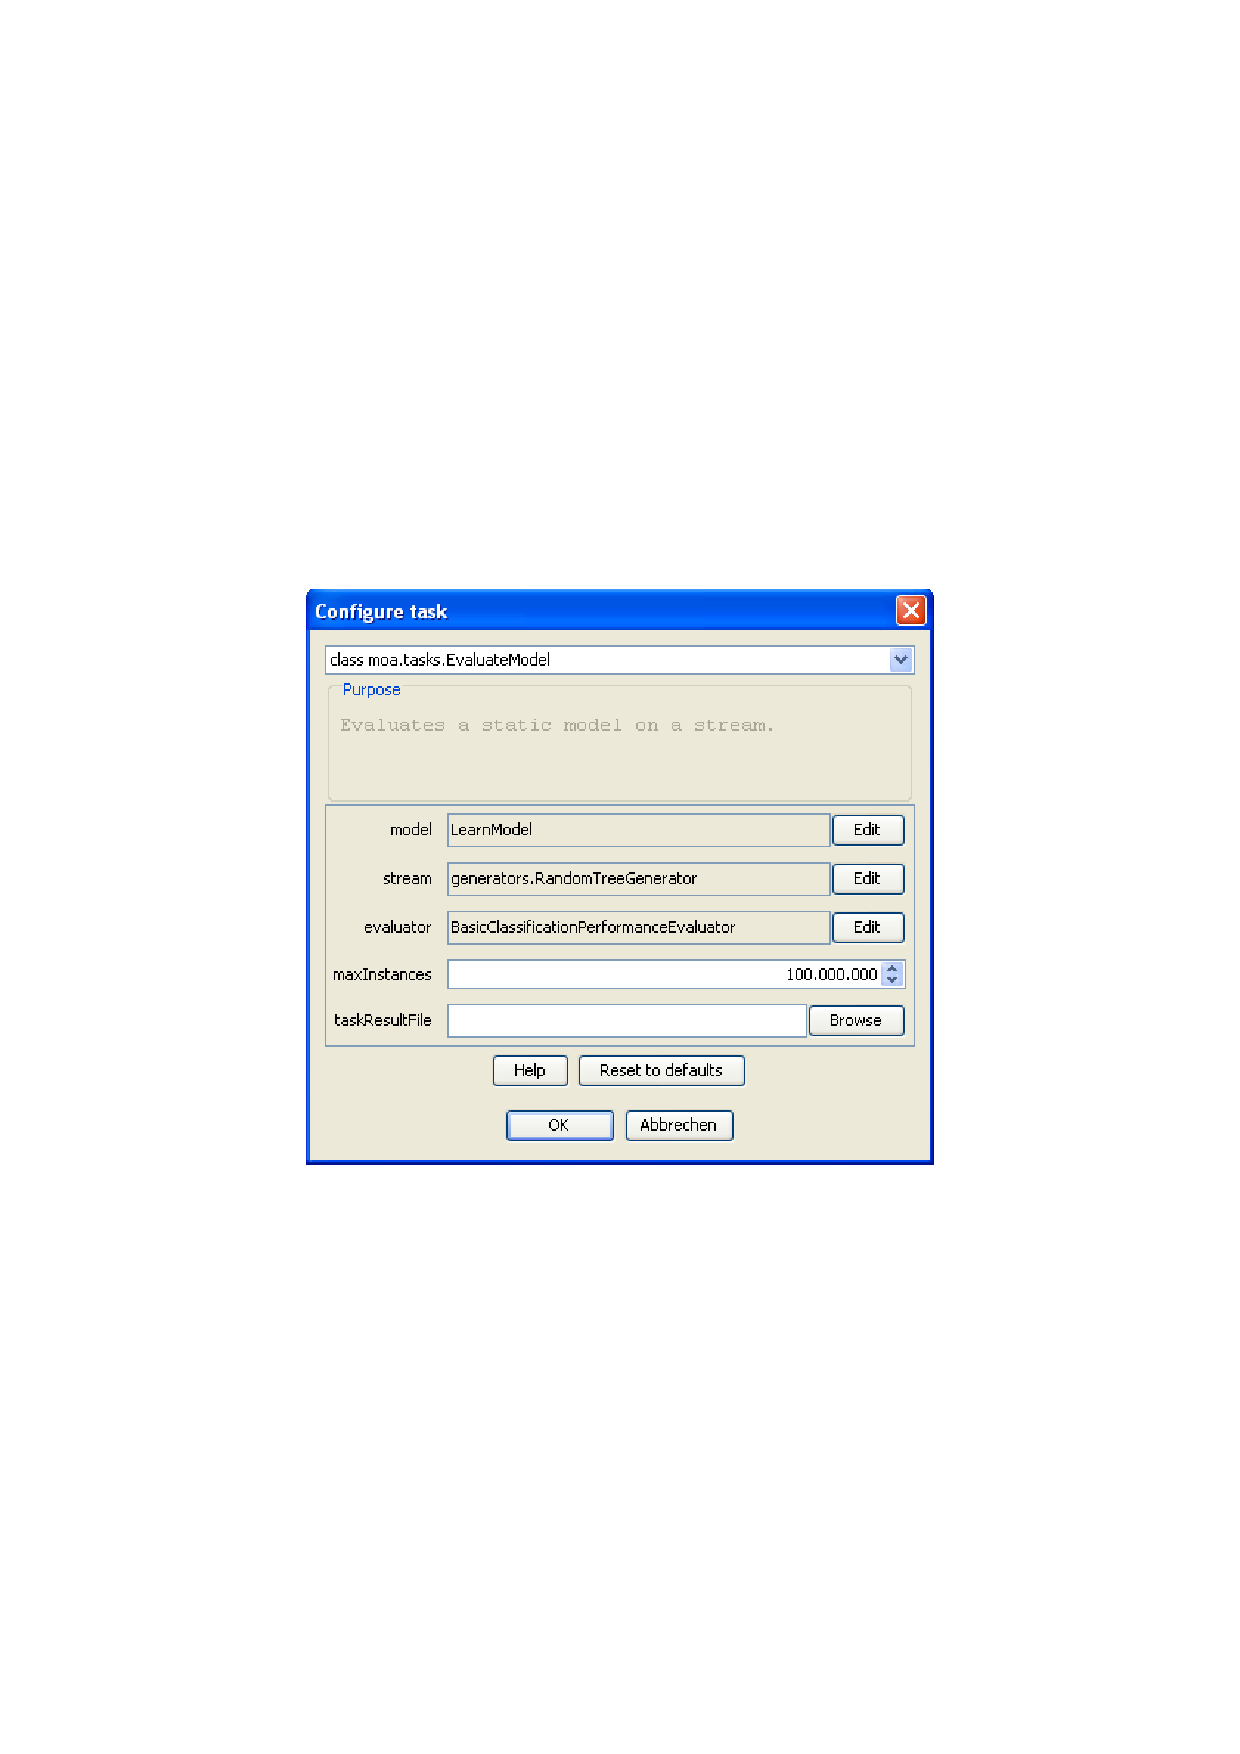
\includegraphics[height=6cm]{images/Configure_Task}\end{center}
\caption{Options to set up a task in MOA}
\end{figure}

\subsection{Regression}

It is now possible to run regression evaluations using the evaluators
\begin{itemize}
\item {\tt BasicRegressionPerformanceEvaluator}  
\item {\tt WindowRegressionPerformanceEvaluator}
\end{itemize}
Currently, it is only possible to use the regressors in the IBLStreams extension of MOA or in WEKA.
See Section~\ref{sec:InstWeka} and Chapter~\ref{chap:Weka} for more information how to use WEKA learners. 


\subsection{Clustering}

The stream clustering tab of MOA has the following main components:
\begin{itemize}
	\item data generators for stream clustering on evolving streams (including events like novelty, merge, etc.),
	\item a set of state-of-the-art stream clustering algorithms,
	\item evaluation measures for stream clustering,
	\item visualization tools for analyzing results and comparing different settings.
\end{itemize}

\subsubsection{Data feeds and data generators}
\label{sec:generators}

\begin{figure}[t]
	\centering
		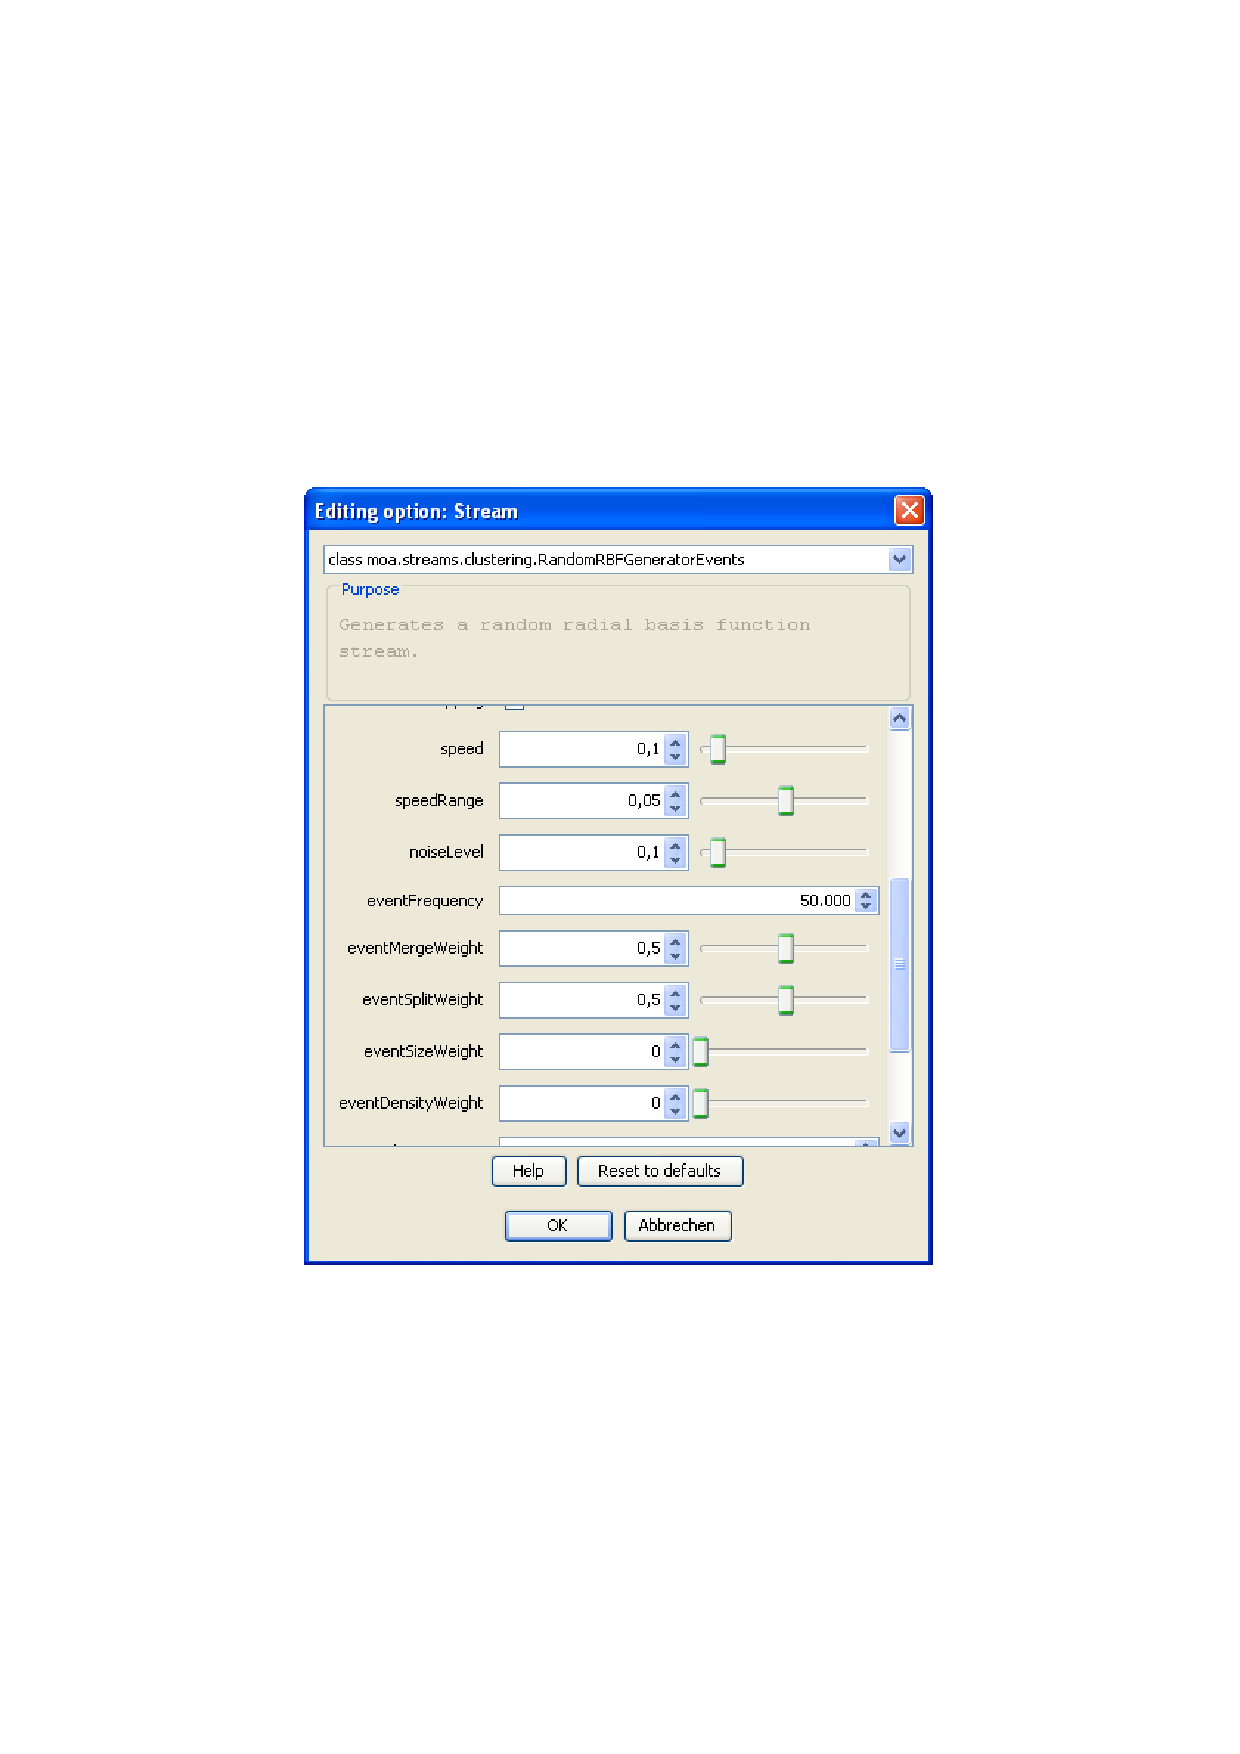
\includegraphics[width=0.55\textwidth]{images/SetupTab}
	\caption{Option dialog for the RBF data generator (by storing and loading settings benchmark streaming data sets can be shared for repeatability and comparison).}
	\label{fig:framework}
\end{figure}
Figure \ref{fig:framework} shows a screenshot of the configuration dialog for the RBF data generator with events. 
Generally the dimensionality, number and size of clusters can be set as well as the drift speed, decay horizon (aging) and noise rate etc.
 Events constitute changes in the underlying data model such as growing of clusters, merging of clusters or creation of new clusters. 
Using the event frequency and the individual event weights, one can study the behaviour and performance of different approaches on various settings. 
Finally, the settings for the data generators can be stored and loaded, which offers the opportunity of sharing settings and thereby providing benchmark streaming data 
sets for repeatability and comparison. 

\subsubsection{Stream clustering algorithms}
\label{sec:algos}

Currently MOA contains several stream clustering methods including:

%\BEGINOMIT
\begin{itemize}
	\item StreamKM++: It computes a small weighted sample of the data stream
	 and it uses the k-means++ algorithm as a randomized seeding technique to choose the 
	 first values for the clusters. To compute the small sample, it employs coreset constructions
	 using a coreset tree for speed up. 
	\item CluStream: It maintains statistical information about the data using micro-clusters. These micro-clusters are temporal extensions of cluster feature vectors. The 
	micro-clusters are stored at snapshots in time following a pyramidal pattern. This pattern 
	allows to recall summary statistics from different time horizons. 
	\item ClusTree: It is a parameter free algorithm automatically adapting to the speed of the stream and it is capable of detecting concept drift, novelty, and outliers in the stream. It uses a compact and self-adaptive index structure for maintaining stream summaries.
	\item Den-Stream: It uses dense micro-clusters (named core-micro-cluster) 
	to summarize clusters. To maintain and distinguish the potential clusters and outliers, 
	this method presents core-micro-cluster and outlier micro-cluster structures.
	  \item CobWeb. One of the first incremental methods for clustering data. 
	  It uses a classification tree. Each node in a classification tree represents a class (concept)
	   and is labeled by a probabilistic concept that summarizes the attribute-value distributions
	    of objects classified under the node. 
\end{itemize}
%\ENDOMIT



\subsubsection{Visualization and analysis}
\label{sec:gui}

After the evaluation process is started, several options for analyzing the outputs are given:
\begin{itemize}
\item the stream can be stopped and the current (micro) clustering result can be passed as a data set to the WEKA explorer for further analysis or mining; 
\item the evaluation measures, which are taken at configurable time intervals, can be stored as a {.csv} file to obtain graphs and charts offline using a program of choice;
\item last but not least both the clustering results and the corresponding measures can be visualized online within MOA.\end{itemize}


MOA allows the simultaneous configuration and evaluation of two different setups for direct comparison, e.g. of two different algorithms 
on the same stream or the same algorithm on streams with different noise levels etc.

\begin{figure*}[t]
\begin{center} 
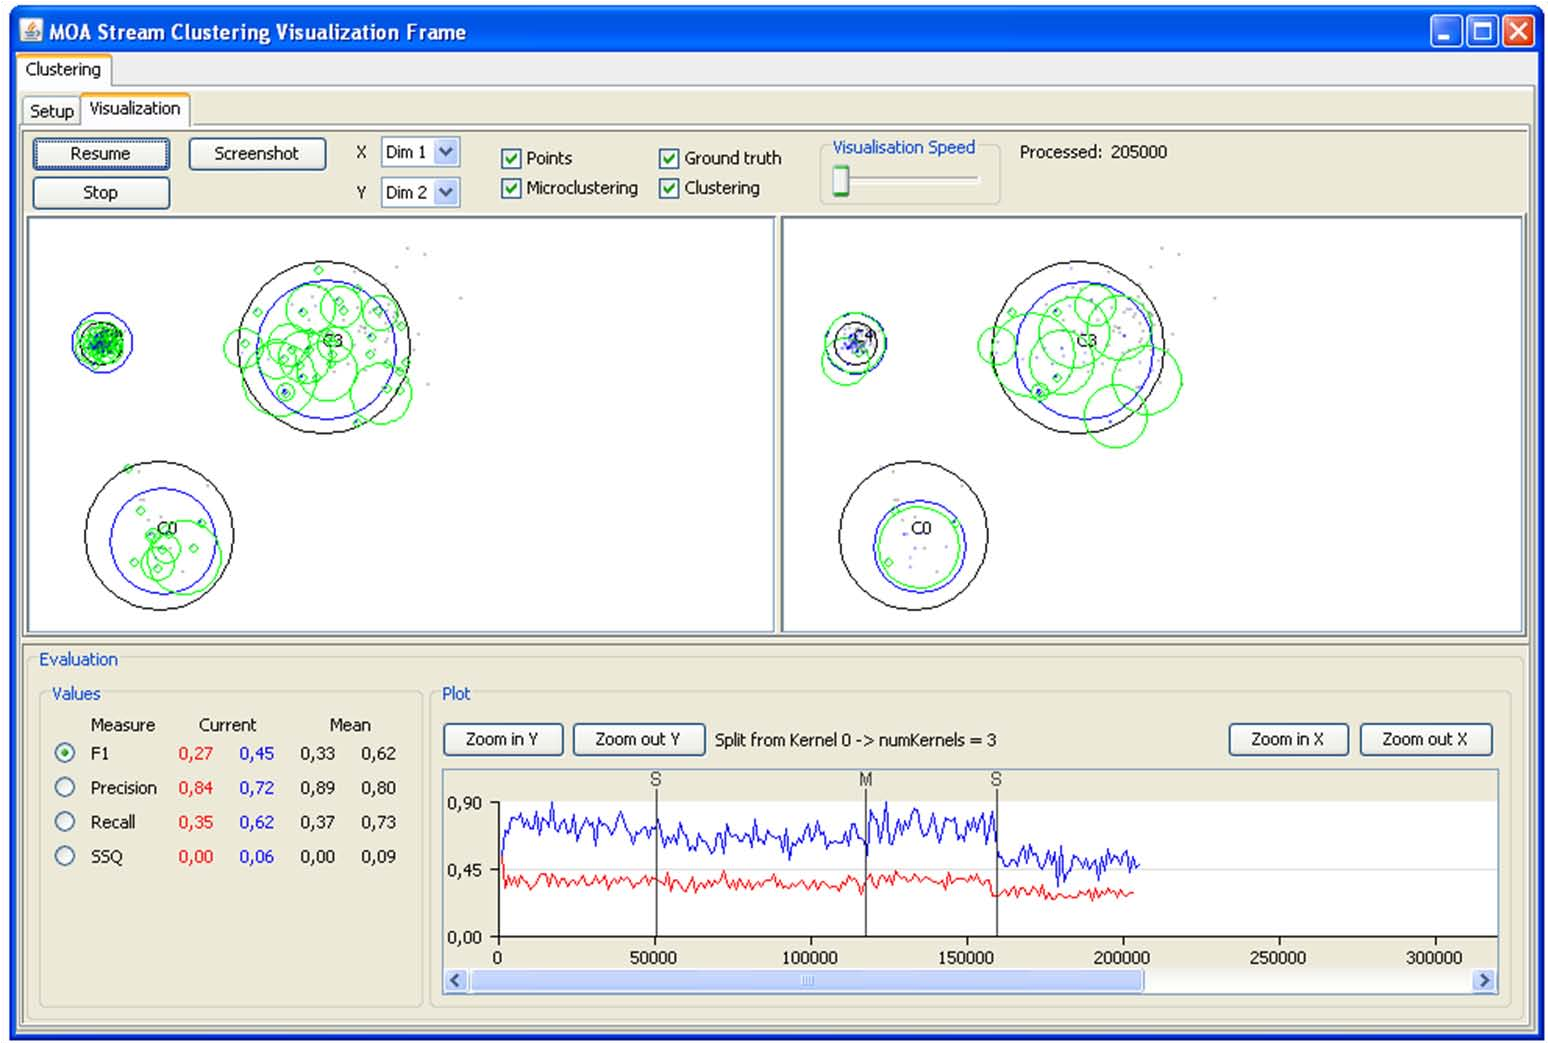
\includegraphics[width=0.9\textwidth]{images/VisualTab}
\end{center} 
\caption{Visualization tab of the clustering MOA graphical user interface.}
\label{fig:VisualTab}
\end{figure*}

The visualization component allows to visualize the stream as well as the clustering results, choose dimensions for multi dimensional settings, and compare experiments with different settings in parallel. 
Figure \ref{fig:VisualTab} shows a screen shot of the visualization tab. 
For this screen shot two different settings of the CluStream algorithm were compared on the same stream setting (including merge/split events every 50000 examples) 
and four measures were chosen for online evaluation (F1, Precision, Recall, and SSQ). 

The upper part of the GUI offers options to pause and resume the stream, adjust the visualization speed, choose the dimensions for x and y as well as the components to be displayed 
(points, micro- and macro clustering and ground truth). The lower part of the GUI displays the measured values for both settings as numbers 
(left side, including mean values) and the currently selected measure as a plot over the arrived examples (right, F1 measure in this example).
 For the given setting one can see a clear drop in the performance after the split event at roughly 160000 examples 
(event details are shown when choosing the corresponding vertical line in the plot). 
While this holds for both settings, the left configuration (red, CluStream with 100 micro clusters) is constantly outperformed by the right configuration 
(blue, CluStream with 20 micro clusters). 



\section{Using the command line}

In this section we are going to show some examples of tasks performed using the command line.

The first example will command MOA to train the \verb+HoeffdingTree+ classifier and create a model. The \verb+moa.DoTask+ class is the main class for running tasks on the command line. It will accept the name of a task followed by any appropriate parameters. The first task used is the \verb+LearnModel+ task. The \verb+-l+ parameter specifies the learner, in this case the \verb+HoeffdingTree+ class. The \verb+-s+ parameter specifies the data stream to learn from, in this case it is
specified  \verb+generators.WaveformGenerator+, which is a data stream generator that produces a three-class learning problem of identifying three types of waveform. The \verb+-m+ option specifies the maximum number of examples to train the learner with, in this case one million examples. The \verb+-O+ option specifies a file to output the resulting model to:

\begin{footnotesize}\begin{verbatim}
java -cp moa.jar -javaagent:sizeofag.jar moa.DoTask \
  LearnModel -l trees.HoeffdingTree \
  -s generators.WaveformGenerator -m 1000000 -O model1.moa
\end{verbatim}\end{footnotesize}

This will create a file named \verb+model1.moa+ that contains the decision stump model that was induced during training.

The next example will evaluate the model to see how accurate it is on a set of examples that are generated using a different random seed. The \verb+EvaluateModel+ task is given the parameters needed to load the model produced in the previous step, generate a new waveform stream with a random seed of 2, and test on one million examples:

\begin{footnotesize}\begin{verbatim}
java -cp moa.jar -javaagent:sizeofag.jar moa.DoTask \
  "EvaluateModel -m file:model1.moa \
  -s (generators.WaveformGenerator -i 2) -i 1000000"
\end{verbatim}\end{footnotesize}

This is the first example of nesting parameters using brackets. Quotes have been added around the description of the task, otherwise the operating system may be confused about the meaning of the brackets.

After evaluation the following statistics are output:

\begin{footnotesize}\begin{verbatim}
classified instances = 1,000,000
classifications correct (percent) = 84.474
Kappa Statistic (percent) = 76.711
\end{verbatim}\end{footnotesize}

Note the the above two steps can be achieved by rolling them into one, avoiding the need to create an external file, as follows:

\begin{footnotesize}\begin{verbatim}
java -cp moa.jar -javaagent:sizeofag.jar moa.DoTask \
  "EvaluateModel -m (LearnModel -l trees.HoeffdingTree \
  -s generators.WaveformGenerator -m 1000000) \
  -s (generators.WaveformGenerator -i 2) -i 1000000"
\end{verbatim}\end{footnotesize}

The task \verb+EvaluatePeriodicHeldOutTest+ will train a model while taking snapshots of performance using a held-out test set at periodic intervals.
The following command creates a {\em comma separated values} file, training the \verb+HoeffdingTree+ classifier on the \verb+WaveformGenerator+ data, using the first 100 thousand examples for testing, training on a total of 100 million examples, and testing every one million examples:

\begin{footnotesize}\begin{verbatim}
java -cp moa.jar -javaagent:sizeofag.jar moa.DoTask \
  "EvaluatePeriodicHeldOutTest -l trees.HoeffdingTree \
  -s generators.WaveformGenerator \
  -n 100000 -i 100000000 -f 1000000" > dsresult.csv
\end{verbatim}\end{footnotesize}

  For the purposes of comparison, a bagging learner using ten decisions trees can be trained on
the same problem:
\begin{footnotesize}\begin{verbatim}
java -cp moa.jar -javaagent:sizeofag.jar moa.DoTask \
  "EvaluatePeriodicHeldOutTest -l (OzaBag -l trees.HoeffdingTree -s 10)\
  -s generators.WaveformGenerator \
  -n 100000 -i 100000000 -f 1000000" > htresult.csv
\end{verbatim}\end{footnotesize}


Another evaluation method implemented in MOA is \emph{Interleaved Test-Then-Train}  or \emph{Prequential}:
 Each individual example is used to test the model
before it is used for training, and from this the accuracy is incrementally
updated. When intentionally performed in this order, the model is always
being tested on examples it has not seen. This scheme has the advantage that
no holdout set is needed for testing, making maximum use of the available
data. It also ensures a smooth plot of accuracy over time, as each individual
example will become increasingly less significant to the overall average.

An example of the EvaluateInterleavedTestThenTrain task  
creating a comma separated values file, training the
HoeffdingTree classifier on the WaveformGenerator data, training and testing on a total of 100 million
examples, and testing every one million examples, is the following:

\begin{footnotesize}\begin{verbatim}
java -cp moa.jar -javaagent:sizeofag.jar moa.DoTask \
  "EvaluateInterleavedTestThenTrain -l trees.HoeffdingTree \
  -s generators.WaveformGenerator \
  -i 100000000 -f 1000000" > htresult.csv
\end{verbatim}
\end{footnotesize}

%\BEGINOMIT
\subsection{Comparing two classifiers}

Suppose we would like to compare the learning curves of a decision stump and a Hoeffding Tree.
First, we will execute the
 task \verb+EvaluatePeriodicHeldOutTest+ to train a model while taking snapshots of performance using a held-out test set at periodic intervals.
The following commands create {\em comma separated values} files, training the \verb+DecisionStump+ and the \verb+HoeffdingTree+ classifier on the \verb+WaveformGenerator+ data, using the first 100 thousand examples for testing, training on a total of 100 million examples, and testing every one million examples:

\begin{footnotesize}\begin{verbatim}
java -cp moa.jar -javaagent:sizeofag.jar moa.DoTask \
  "EvaluatePeriodicHeldOutTest -l trees.DecisionStump \
  -s generators.WaveformGenerator \
  -n 100000 -i 100000000 -f 1000000" > dsresult.csv
\end{verbatim}\end{footnotesize}

\begin{footnotesize}\begin{verbatim}
java -cp moa.jar -javaagent:sizeofag.jar moa.DoTask \
  "EvaluatePeriodicHeldOutTest -l trees.HoeffdingTree \
  -s generators.WaveformGenerator \
  -n 100000 -i 100000000 -f 1000000" > htresult.csv
\end{verbatim}\end{footnotesize}

Assuming that \verb+gnuplot+ is installed on the system, the learning curves can be plotted with the following commands:

\begin{footnotesize}\begin{verbatim}
gnuplot> set datafile separator ","
gnuplot> set ylabel "% correct"
gnuplot> set xlabel "examples processed"
gnuplot> plot [][0:100] \
  "dsresult.csv" using 1:9 with linespoints \
  title "DecisionStumpTutorial", \
  "htresult.csv" using 1:9 with linespoints \
  title "HoeffdingTree"
\end{verbatim}\end{footnotesize}

This results in the following graph:

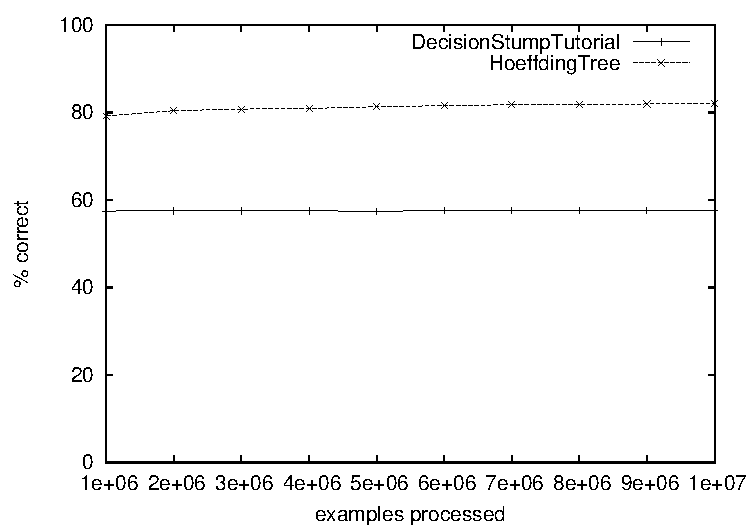
\includegraphics{images/gnuplotGraph}

For this problem it is obvious that a full tree can achieve higher accuracy than a single stump, and that a stump has very stable accuracy that does not improve with further training.
%\ENDOMIT



\chapter{Using the API} %Writing a classifier}

It's easy to use the methods of MOA inside Java Code. For example, this is the Java code for a prequential evaluation:

\begin{lstlisting}[caption={Java Code Example},label=lst:fullclassifier]
int numInstances=10000;

Classifier learner = new HoeffdingTree();
RandomRBFGenerator stream = new RandomRBFGenerator();
stream.prepareForUse();

learner.setModelContext(stream.getHeader());
learner.prepareForUse();

int numberSamplesCorrect=0;
int numberSamples=0;
boolean isTesting = true;
while(stream.hasMoreInstances() && numberSamples < numInstances){
    Instance trainInst = stream.nextInstance();
    if(isTesting){
	if(learner.correctlyClassifies(trainInst)){
	    numberSamplesCorrect++;
	}
    }
    numberSamples++;
    learner.trainOnInstance(trainInst);
}
double accuracy = 100.0*(double) numberSamplesCorrect / (double)numberSamples;
System.out.println(numberSamples+" instances processed with "+accuracy+"% accuracy");
\end{lstlisting}


\section{Creating a new classifier}

To demonstrate the implementation and operation of learning algorithms in the system, the Java code of a simple decision stump classifier is studied. The classifier monitors the result of splitting on each attribute and chooses the attribute the seems to best separate the classes, based on information gain. The decision is revisited many times, so the stump has potential to change over time as more examples are seen. In practice it is unlikely to change after sufficient training.

To describe the implementation, relevant code fragments are discussed in turn, with the entire code listed (Listing~\ref{lst:fullclassifier}) at the end. The line numbers from the fragments match up with the final listing.

A simple approach to writing a classifier is to extend  \\ \verb+moa.classifiers.AbstractClassifier+ (line 10), which will take care of certain details to ease the task.

\begin{lstlisting}[caption={Option handling},label=lst:opthandle,firstnumber=14]
	public IntOption gracePeriodOption = new IntOption("gracePeriod", 'g',
			"The number of instances to observe between model changes.",
			1000, 0, Integer.MAX_VALUE);

	public FlagOption binarySplitsOption = new FlagOption("binarySplits", 'b',
			"Only allow binary splits.");

	public ClassOption splitCriterionOption = new ClassOption("splitCriterion",
			'c', "Split criterion to use.", SplitCriterion.class,
			"InfoGainSplitCriterion");
\end{lstlisting}

To set up the public interface to the classifier, the options available to the user must be specified. For the system to automatically take care of option handling, the options need to be public members of the class, that extend the \verb+moa.options.Option+ type.

The decision stump classifier example has three options, each of a different type.
The meaning of the first three parameters used to construct options are consistent between different option types. The first parameter is a short name used to identify the option. The second is a character intended to be used on the command line. It should be unique---a command line character cannot be repeated for different options otherwise an exception will be thrown. The third standard parameter is a string describing the purpose of the option. Additional parameters to option constructors allow things such as default values and valid ranges to be specified.

The first option specified for the decision stump classifier is the ``grace period''. The option is expressed with an integer, so the option has the type \verb+IntOption+. The parameter will control how frequently the best stump is reconsidered when learning from a stream of examples. This increases the efficiency of the classifier---evaluating after every single example is expensive, and it is unlikely that a single example will change the decision of the current best stump. The default value of 1000 means that the choice of stump will be re-evaluated only after 1000 examples have been observed since the last evaluation. The last two parameters specify the range of values that are allowed for the option---it makes no sense to have a negative grace period, so the range is restricted to integers 0 or greater.

The second option is a flag, or a binary switch, represented by a \\ \verb+FlagOption+. By default all flags are turned off, and will be turned on only when a user requests so. This flag controls whether the decision stumps should only be allowed to split two ways. By default the stumps are allowed have more than two branches.

The third option determines the split criterion that is used to decide which stumps are the best. This is a \verb+ClassOption+ that requires a particular Java class of the type \verb+SplitCriterion+. If the required class happens to be an \verb+OptionHandler+ then those options will be used to configure the object that is passed in.

\begin{lstlisting}[caption={Miscellaneous fields},label=lst:miscfields,firstnumber=25]
	protected AttributeSplitSuggestion bestSplit;

	protected DoubleVector observedClassDistribution;

	protected AutoExpandVector<AttributeClassObserver> attributeObservers;

	protected double weightSeenAtLastSplit;

	public boolean isRandomizable() {
		return false;
	}
\end{lstlisting}

Four global variables are used to maintain the state of the classifier.

The \verb+bestSplit+ field maintains the current stump that has been chosen by the classifier. It is of type \verb+AttributeSplitSuggestion+, a class used to split instances into different subsets.

The \verb+observedClassDistribution+ field remembers the overall distribution of class labels that have been observed by the classifier. It is of type \verb+DoubleVector+, which is a handy class for maintaining a vector of floating point values without having to manage its size.

The \verb+attributeObservers+ field stores a collection of \\ \verb+AttributeClassObserver+s, one for each attribute. This is the information needed to decide which attribute is best to base the stump on.

The \verb+weightSeenAtLastSplit+ field records the last time an evaluation was performed, so that it can be determined when another evaluation is due, depending on the grace period parameter.

The \verb+isRandomizable()+ function needs to be implemented to specify whether the classifier has an element of randomness. If it does, it will automatically be set up to accept a random seed. This classifier is does not, so \verb+false+ is returned.

\begin{lstlisting}[caption={Preparing for learning},label=lst:preplearn,firstnumber=37]
	@Override
	public void resetLearningImpl() {
		this.bestSplit = null;
		this.observedClassDistribution = new DoubleVector();
		this.attributeObservers = new AutoExpandVector<AttributeClassObserver>();
		this.weightSeenAtLastSplit = 0.0;
	}
\end{lstlisting}

This function is called before any learning begins, so it should set the default state when no information has been supplied, and no training examples have been seen. In this case, the four global fields are set to sensible defaults.

\begin{lstlisting}[caption={Training on examples},label=lst:train,firstnumber=45]
	@Override
	public void trainOnInstanceImpl(Instance inst) {
		this.observedClassDistribution.addToValue((int) inst.classValue(), inst
				.weight());
		for (int i = 0; i < inst.numAttributes() - 1; i++) {
			int instAttIndex = modelAttIndexToInstanceAttIndex(i, inst);
			AttributeClassObserver obs = this.attributeObservers.get(i);
			if (obs == null) {
				obs = inst.attribute(instAttIndex).isNominal() ?
					newNominalClassObserver() : newNumericClassObserver();
				this.attributeObservers.set(i, obs);
			}
			obs.observeAttributeClass(inst.value(instAttIndex), (int) inst
					.classValue(), inst.weight());
		}
		if (this.trainingWeightSeenByModel - this.weightSeenAtLastSplit >=
				this.gracePeriodOption.getValue()) {
			this.bestSplit = findBestSplit((SplitCriterion)
				getPreparedClassOption(this.splitCriterionOption));
			this.weightSeenAtLastSplit = this.trainingWeightSeenByModel;
		}
	}
\end{lstlisting}

This is the main function of the learning algorithm, called for every training example in a stream. The first step, lines 47-48, updates the overall recorded distribution of classes. The loop from line 49 to line 59 repeats for every attribute in the data. If no observations for a particular attribute have been seen previously, then lines 53-55 create a new observing object. Lines 57-58 update the observations with the values from the new example. Lines 60-61 check to see if the grace period has expired. If so, the best split is re-evaluated.

\begin{lstlisting}[caption={Functions used during training},label=lst:trainfuncs,firstnumber=79]
	protected AttributeClassObserver newNominalClassObserver() {
		return new NominalAttributeClassObserver();
	}

	protected AttributeClassObserver newNumericClassObserver() {
		return new GaussianNumericAttributeClassObserver();
	}

	protected AttributeSplitSuggestion findBestSplit(SplitCriterion criterion) {
		AttributeSplitSuggestion bestFound = null;
		double bestMerit = Double.NEGATIVE_INFINITY;
		double[] preSplitDist = this.observedClassDistribution.getArrayCopy();
		for (int i = 0; i < this.attributeObservers.size(); i++) {
			AttributeClassObserver obs = this.attributeObservers.get(i);
			if (obs != null) {
				AttributeSplitSuggestion suggestion =
					obs.getBestEvaluatedSplitSuggestion(
						criterion,
						preSplitDist,
						i,
						this.binarySplitsOption.isSet());
				if (suggestion.merit > bestMerit) {
					bestMerit = suggestion.merit;
					bestFound = suggestion;
				}
			}
		}
		return bestFound;
	}
\end{lstlisting}

These functions assist the training algorithm. \\ \verb+newNominalClassObserver+ and \verb+newNumericClassObserver+ are responsible for creating new observer objects for nominal and numeric attributes, respectively. The \verb+findBestSplit()+ function will iterate through the possible stumps and return the one with the highest `merit' score.

\begin{lstlisting}[caption={Predicting class of unknown examples},label=lst:test,firstnumber=68]
	public double[] getVotesForInstance(Instance inst) {
		if (this.bestSplit != null) {
			int branch = this.bestSplit.splitTest.branchForInstance(inst);
			if (branch >= 0) {
				return this.bestSplit
						.resultingClassDistributionFromSplit(branch);
			}
		}
		return this.observedClassDistribution.getArrayCopy();
	}
\end{lstlisting}

This is the other important function of the classifier besides training---using the model that has been induced to predict the class of examples. For the decision stump, this involves calling the functions \verb+branchForInstance()+ and \verb+resultingClassDistributionFromSplit()+ that are implemented by the \verb+AttributeSplitSuggestion+ class.

Putting all of the elements together, the full listing of the tutorial class is given below.

\begin{lstlisting}[caption={Full listing},label=lst:fullclassifier]
package moa.classifiers;

import moa.core.AutoExpandVector;
import moa.core.DoubleVector;
import moa.options.ClassOption;
import moa.options.FlagOption;
import moa.options.IntOption;
import weka.core.Instance;

public class DecisionStumpTutorial extends AbstractClassifier {

	private static final long serialVersionUID = 1L;

	public IntOption gracePeriodOption = new IntOption("gracePeriod", 'g',
			"The number of instances to observe between model changes.",
			1000, 0, Integer.MAX_VALUE);

	public FlagOption binarySplitsOption = new FlagOption("binarySplits", 'b',
			"Only allow binary splits.");

	public ClassOption splitCriterionOption = new ClassOption("splitCriterion",
			'c', "Split criterion to use.", SplitCriterion.class,
			"InfoGainSplitCriterion");

	protected AttributeSplitSuggestion bestSplit;

	protected DoubleVector observedClassDistribution;

	protected AutoExpandVector<AttributeClassObserver> attributeObservers;

	protected double weightSeenAtLastSplit;

	public boolean isRandomizable() {
		return false;
	}

	@Override
	public void resetLearningImpl() {
		this.bestSplit = null;
		this.observedClassDistribution = new DoubleVector();
		this.attributeObservers = new AutoExpandVector<AttributeClassObserver>();
		this.weightSeenAtLastSplit = 0.0;
	}

	@Override
	public void trainOnInstanceImpl(Instance inst) {
		this.observedClassDistribution.addToValue((int) inst.classValue(), inst
				.weight());
		for (int i = 0; i < inst.numAttributes() - 1; i++) {
			int instAttIndex = modelAttIndexToInstanceAttIndex(i, inst);
			AttributeClassObserver obs = this.attributeObservers.get(i);
			if (obs == null) {
				obs = inst.attribute(instAttIndex).isNominal() ?
					newNominalClassObserver() : newNumericClassObserver();
				this.attributeObservers.set(i, obs);
			}
			obs.observeAttributeClass(inst.value(instAttIndex), (int) inst
					.classValue(), inst.weight());
		}
		if (this.trainingWeightSeenByModel - this.weightSeenAtLastSplit >=
				this.gracePeriodOption.getValue()) {
			this.bestSplit = findBestSplit((SplitCriterion)
				getPreparedClassOption(this.splitCriterionOption));
			this.weightSeenAtLastSplit = this.trainingWeightSeenByModel;
		}
	}

	public double[] getVotesForInstance(Instance inst) {
		if (this.bestSplit != null) {
			int branch = this.bestSplit.splitTest.branchForInstance(inst);
			if (branch >= 0) {
				return this.bestSplit
						.resultingClassDistributionFromSplit(branch);
			}
		}
		return this.observedClassDistribution.getArrayCopy();
	}

	protected AttributeClassObserver newNominalClassObserver() {
		return new NominalAttributeClassObserver();
	}

	protected AttributeClassObserver newNumericClassObserver() {
		return new GaussianNumericAttributeClassObserver();
	}

	protected AttributeSplitSuggestion findBestSplit(SplitCriterion criterion) {
		AttributeSplitSuggestion bestFound = null;
		double bestMerit = Double.NEGATIVE_INFINITY;
		double[] preSplitDist = this.observedClassDistribution.getArrayCopy();
		for (int i = 0; i < this.attributeObservers.size(); i++) {
			AttributeClassObserver obs = this.attributeObservers.get(i);
			if (obs != null) {
				AttributeSplitSuggestion suggestion =
					obs.getBestEvaluatedSplitSuggestion(
						criterion,
						preSplitDist,
						i,
						this.binarySplitsOption.isSet());
				if (suggestion.merit > bestMerit) {
					bestMerit = suggestion.merit;
					bestFound = suggestion;
				}
			}
		}
		return bestFound;
	}

	public void getModelDescription(StringBuilder out, int indent) {
	}

	protected moa.core.Measurement[] getModelMeasurementsImpl() {
		return null;
	}

}
\end{lstlisting}



\section{Compiling a classifier}

The following five files are assumed to be in the current working directory:

\begin{verbatim}
DecisionStumpTutorial.java
moa.jar
sizeofag.jar
\end{verbatim}

The example source code can be compiled with the following command:

\begin{verbatim}
javac -cp moa.jar DecisionStumpTutorial.java
\end{verbatim}

This produces compiled java class file \verb+DecisionStumpTutorial.class+.

Before continuing, the commands below set up directory structure to reflect the package structure:

\begin{verbatim}
mkdir moa
mkdir moa/classifiers
cp DecisionStumpTutorial.class moa/classifiers/
\end{verbatim}

The class is now ready to use.



\chapter{Tasks in MOA}

The main Tasks in MOA are the following:



\section{WriteStreamToARFFFile} 

Outputs a stream to an ARFF file. 
Example:
\begin{footnotesize}\begin{verbatim}
java -cp moa.jar -javaagent:sizeofag.jar moa.DoTask \
  "WriteStreamToARFFFile -s generators.WaveformGenerator \
  -f Wave.arff -m 100000" 
\end{verbatim}\end{footnotesize}

Parameters:
\begin{itemize}
\item -s : Stream to write
\item -f : Destination ARFF file
\item -m : Maximum number of instances to write to file
\item -h : Suppress header from output\end{itemize}

\section{MeasureStreamSpeed} 
Measures the speed of a stream. Example:

\begin{footnotesize}\begin{verbatim}
java -cp moa.jar -javaagent:sizeofag.jar moa.DoTask \
  "MeasureStreamSpeed -s generators.WaveformGenerator \
  -g 100000" 
\end{verbatim}\end{footnotesize}

Parameters:
\begin{itemize}
\item -s : Stream to measure
\item -g : Number of examples
\item -O : File to save the final result of the task to
\end{itemize}

\section{LearnModel} 
Learns a model from a stream.
Example:
\begin{footnotesize}\begin{verbatim}
java -cp moa.jar -javaagent:sizeofag.jar moa.DoTask \
  LearnModel -l trees.HoeffdingTree \
  -s generators.WaveformGenerator -m 1000000 -O model1.moa
\end{verbatim}\end{footnotesize}

Parameters:
\begin{itemize}
\item -l : Classifier to train
\item -s : Stream to learn from
\item -m : Maximum number of instances to train on per pass over the data
\item -p : The number of passes to do over the data
\item -b : Maximum size of model (in bytes). -1 = no limit
\item -q : How many instances between memory bound checks
\item -O : File to save the final result of the task to
\end{itemize}

\section{EvaluateModel} 
Evaluates a static model on a stream.
Example:
\begin{footnotesize}\begin{verbatim}
java -cp moa.jar -javaagent:sizeofag.jar moa.DoTask \
  "EvaluateModel -m (LearnModel -l trees.HoeffdingTree \
  -s generators.WaveformGenerator -m 1000000) \
  -s (generators.WaveformGenerator -i 2) -i 1000000"
\end{verbatim}\end{footnotesize}

Parameters:
\begin{itemize}
\item -l : Classifier to evaluate
\item -s : Stream to evaluate on
\item -e : Classification performance evaluation method
\item -i : Maximum number of instances to test
\item -O : File to save the final result of the task to
\end{itemize}

\section{EvaluatePeriodicHeldOutTest}

Evaluates a classifier on a stream by periodically testing on a heldout set.
Example:
\begin{footnotesize}\begin{verbatim}
java -cp moa.jar -javaagent:sizeofag.jar moa.DoTask \
  "EvaluatePeriodicHeldOutTest -l trees.HoeffdingTree \
  -s generators.WaveformGenerator \
  -n 100000 -i 100000000 -f 1000000" > htresult.csv
\end{verbatim}\end{footnotesize}

Parameters:
\begin{itemize}
\item -l : Classifier to train
\item -s : Stream to learn from
\item -e : Classification performance evaluation method
\item -n : Number of testing examples
\item -i : Number of training examples, $<$1 = unlimited
\item -t : Number of training seconds
\item -f : Number of training examples between samples of learning performance
\item -d : File to append intermediate csv results to
\item -c : Cache test instances in memory
\item -O : File to save the final result of the task to
\end{itemize}

\section{EvaluateInterleavedTestThenTrain}
Evaluates a classifier on a stream by testing then training with each example in sequence.
Example:
\begin{footnotesize}\begin{verbatim}
java -cp moa.jar -javaagent:sizeofag.jar moa.DoTask \
  "EvaluateInterleavedTestThenTrain -l trees.HoeffdingTree \
  -s generators.WaveformGenerator \
  -i 100000000 -f 1000000" > htresult.csv
\end{verbatim}
\end{footnotesize}

Parameters:
\begin{itemize}
\item -l : Classifier to train
\item -s : Stream to learn from
\item -e : Classification performance evaluation method
\item -i : Maximum number of instances to test/train on  (-1 = no limit)
\item -t : Maximum number of seconds to test/train for (-1 = no limit)
\item -f : How many instances between samples of the learning performance
\item -b : Maximum size of model (in bytes). -1 = no limit
\item -q : How many instances between memory bound checks
\item -d : File to append intermediate csv results to
\item -O : File to save the final result of the task to
\end{itemize}



\section{EvaluatePrequential}
 Evaluates a classifier on a stream by testing then training with each example in sequence.
It may use a sliding window or a fading factor forgetting mechanism.

This evaluation method using sliding windows and a fading factor was presented in

\begin{itemize}
\bibitem[C]{gama}
Jo{\~a}o Gama, Raquel Sebasti{\~a}o and Pedro Pereira Rodrigues.
\newblock Issues in evaluation of stream learning algorithms.
\newblock In {\em KDD'09}, pages 329--338.\end{itemize}

The fading factor $\alpha$ is used as following:
$$E_i = \frac{S_i} {B_i}$$
with
 $$S_i = L_i + \alpha \times S_{i-1}$$ $$B_i = n_i + \alpha \times B_{i-1}$$
where $n_i$ is the number of examples used to compute the loss function $L_i$.
$n_i = 1$ since the loss $L_i$ is computed for every single example.


Examples:
\begin{footnotesize}\begin{verbatim}
java -cp moa.jar -javaagent:sizeofag.jar moa.DoTask \
  "EvaluatePrequential -l trees.HoeffdingTree \
  -e (WindowClassificationPerformanceEvaluator -w 10000) \
  -s generators.WaveformGenerator \
  -i 100000000 -f 1000000" > htresult.csv
\end{verbatim}
\begin{verbatim}
java -cp moa.jar -javaagent:sizeofag.jar moa.DoTask \
  "EvaluatePrequential -l trees.HoeffdingTree \
  -e (FadingFactorClassificationPerformanceEvaluator -a .975) \
  -s generators.WaveformGenerator \
  -i 100000000 -f 1000000" > htresult.csv
\end{verbatim}

\end{footnotesize}

Parameters:
\begin{itemize}
 \item Same parameters as EvaluateInterleavedTestThenTrain
\item -e : Classification performance evaluation method
\begin{itemize}
 \item WindowClassificationPerformanceEvaluator
\begin{itemize}
\item -w : Size of sliding window to use with WindowClassificationPerformanceEvaluator
\end{itemize}
 \item FadingFactorClassificationPerformanceEvaluator
\begin{itemize}
\item -a : Fading factor to use with FadingFactorClassificationPerformanceEvaluator
\end{itemize}
 \item EWMAFactorClassificationPerformanceEvaluator
\begin{itemize}
\item -a : Fading factor to use with FadingFactorClassificationPerformanceEvaluator
\end{itemize}
\end{itemize}
\end{itemize}

\section{EvaluateInterleavedChunks}

Evaluates a classifier on a stream by testing then training with chunks of data in sequence.

Parameters:
\begin{itemize}
\item -l : Classifier to train
\item -s : Stream to learn from
\item -e : Classification performance evaluation method
\item -i : Maximum number of instances to test/train on  (-1 = no limit)
\item -c : Number of instances in a data chunk.
\item -t : Maximum number of seconds to test/train for (-1 = no limit)
\item -f : How many instances between samples of the learning performance
\item -b : Maximum size of model (in bytes). -1 = no limit
\item -q : How many instances between memory bound checks
\item -d : File to append intermediate csv results to
\item -O : File to save the final result of the task to
\end{itemize}


\chapter{Evolving data streams}

MOA streams are build using generators, reading ARFF files, joining several streams, or filtering streams.
MOA streams generators allow to simulate potentially infinite sequence of data. 
There are the following :
\begin{itemize}
\item Random Tree Generator
\item SEA Concepts Generator
\item STAGGER Concepts Generator
\item Rotating Hyperplane
\item Random RBF Generator
\item LED Generator
\item Waveform Generator
\item Function Generator
\end{itemize}
.

\section{Streams}

Classes available in MOA to obtain input streams are the following:

\subsection{ArffFileStream}
 A stream read from an ARFF file.
 Example:
\begin{footnotesize}
\begin{verbatim}               
   ArffFileStream -f elec.arff
\end{verbatim} \end{footnotesize}

Parameters:

\begin{itemize}
\item 
-f : ARFF file to load
\item -c : Class index of data. 0 for none or -1 for last attribute in file\end{itemize}


\subsection{ConceptDriftStream}
 Generator that adds concept drift to examples in a stream.

Considering data streams as data generated from pure distributions, MOA models
a concept drift {event} as a weighted combination %a mixture distribution, 
of two pure distributions that characterizes the target concepts before and after
the drift.  MOA uses 
the sigmoid function, as an elegant and practical solution to define the probability that every new 
instance of the stream belongs to the new concept after the drift.

\begin{figure}
\begin{tikzpicture}[domain=-2:9]
  \draw[step=2,very thin,color=gray] (-0.1,-0.1) grid (8.2,4.2);
  \draw[->] (-2.2,0) -- (8.2,0) node[right] {$t$};
  \draw[->] (0,-0.2) -- (0,4.2) node[above] {$f(t)$};
  \draw[<->] (2,-0.6) -- (6,-0.6) node[below] {};
  \draw[color=blue!50!black, domain=2:6] plot[id=x]   function{(x-2)}           node[right]{}; %{$f(x) =x$};
  \draw[color=red!50!black] plot[id=exp] function{4/(1+exp(4-x))} node[right] {$f(t)$};% = 1/{(1+ \mathrm e^{-s (x-x_0)}})$};
  \colorlet{anglecolor}{blue!50!black}
  \filldraw[fill=blue!20,draw=anglecolor] (2,0) -- (2.5,0) arc(0:45:.5);
  \draw (2.7,.3) node[anglecolor] {$\alpha$};
  \filldraw[fill=blue!20,draw=anglecolor] (4,2) -- (4.5,2) arc(0:45:.5);
  \draw (4.7,2.3) node[anglecolor] {$\alpha$};

  \draw (4,-0.3) node[] {$t_0$};
  \draw (4,-0.9) node[] {$W$};
  \draw (-0.5,2) node[] {$0.5$};
  \draw (-0.5,4) node[] {$1$};

\end{tikzpicture}
\caption{A sigmoid function $f(t) = 1/{(1+ \mathrm e^{-s (t-t_0)}})$.}
\label{fig:ConceptChange}
\end{figure}

We see from Figure~\ref{fig:ConceptChange} that the sigmoid function 
$$f(t) = 1/{(1+ \mathrm e^{-s (t-t_0)}})$$
has a derivative at the point $t_0$ equal to $f'(t_0) = s/4$. The tangent of angle 
$\alpha$ is equal to this derivative, $\tan \alpha = s/4$. We observe that 
$ \tan \alpha = 1/ W$,
and as $s= 4 \tan \alpha$ then $s=4/W$. So the parameter $s$ in the sigmoid 
gives the length of $W$ and the angle $\alpha$. 
In this sigmoid model we only need to specify two parameters : 
$t_0$ the point of change, and $W$ the length of change.
Note that for any positive real number $\beta$ $$f(t_0+\beta \cdot W)=1 -f(t_0-\beta \cdot W),$$ and  that $f(t_0+\beta \cdot W)$ and $f(t_0-\beta \cdot W)$ 
are constant values that don't depend on $t_0$ and $W$: 
$$f(t_0+W/2) = 1 - f(t_0-W/2) = 1/( 1+ e^{-2}) \approx 88.08 \%$$  
$$f(t_0+W) = 1 - f(t_0-W) = 1/( 1+ e^{-4}) \approx 98.20 \%$$  
$$f(t_0+2W) = 1 - f(t_0-2W) = 1/( 1+ e^{-8}) \approx 99.97 \%$$
\begin{definition}
Given two data streams $a$, $b$, we define $c = a  \oplus^{W}_{t_0} b$ as the 
data stream built joining the two data streams $a$ and $b$, where
$t_0$ is the point of change, $W$ is the length of change and 
\begin{itemize}
 \item $\Pr[ c(t) = a(t)] = \mathrm e^{-4(t-t_0)/W}/{(1+ \mathrm e^{-4(t-t_0)/W})}$
 \item $\Pr[ c(t) = b(t)] = 1/{(1+ \mathrm e^{-4(t-t_0)/W})}$.
\end{itemize}
\end{definition}

\BEGINOMIT
We observe the following properties, if $a \ne b$:
\begin{itemize}
 \item $a \oplus^{W}_{t_0} b \neq b \oplus^{W}_{t_0} a$
 \item $a \oplus^{W}_{t_0} a = a$
 \item $a \oplus^{0}_{0} b = b$
 \item $a \oplus^{W}_{t_0} ( b \oplus^{W}_{t_0} c) \neq (a \oplus^{W}_{t_0}  b)
	 \oplus^{W}_{t_0} c$
 \item $a \oplus^{W}_{t_0} ( b \oplus^{W}_{t_1} c) \approx (a \oplus^{W}_{t_0}  b)
	 \oplus^{W}_{t_1} c$ if $t_0<t_1$ and $W \ll |t_1-t_0|$
\end{itemize}
In order to create a data stream with multiple concept changes, we can build new 
data streams joining different concept drifts:
$$( ( (a \oplus^{W_0}_{t_0}  b) \oplus^{W_1}_{t_1} c) \oplus^{W_2}_{t_2} d ) \ldots $$ 
\ENDOMIT

Example:
\begin{footnotesize}\begin{verbatim}
 ConceptDriftStream -s (generators.AgrawalGenerator -f 7) 
    -d (generators.AgrawalGenerator -f 2) -w 1000000 -p 900000 
\end{verbatim}\end{footnotesize}
Parameters:

\begin{itemize}
\item -s : Stream 
\item -d : Concept drift Stream
\item -p : Central position of concept drift change
\item -w : Width of concept drift change\end{itemize}


\subsection{ConceptDriftRealStream} Generator that adds concept drift to examples in a stream with 
 different classes and attributes. Example: real datasets

 Example:
\begin{footnotesize}
\begin{verbatim}               
 ConceptDriftRealStream -s (ArffFileStream -f covtype.arff) \
    -d (ConceptDriftRealStream -s (ArffFileStream -f PokerOrig.arff) \
    -d (ArffFileStream -f elec.arff) -w 5000 -p 1000000 ) -w 5000 -p 581012 
\end{verbatim} \end{footnotesize}
Parameters:

\begin{itemize}
\item -s : Stream 
\item -d : Concept drift Stream
\item -p : Central position of concept drift change
\item -w : Width of concept drift change\end{itemize}


\subsection{FilteredStream} A stream that is filtered.

Parameters:

\begin{itemize}
\item -s : Stream to filter 
\item -f : Filters to apply : AddNoiseFilter\end{itemize}


\subsection{AddNoiseFilter} Adds random noise to examples in a stream. Only to use with FilteredStream.

Parameters:

\begin{itemize}
\item -r : Seed for random noise 
\item -a : The fraction of attribute values to disturb
\item -c : The fraction of class labels to disturb\end{itemize}

\section{Streams Generators}
	
The classes available to generate streams are the following:

\subsection{generators.AgrawalGenerator} Generates one of ten different pre-defined loan functions

It was introduced by Agrawal et al. in
\begin{itemize}
\bibitem[A]{agrawal93}
R.~Agrawal, T.~Imielinski, and A.~Swami.
\newblock Database mining: A performance perspective.
\newblock {\em IEEE Trans. on Knowl. and Data Eng.}, 5(6):914--925, 1993.\end{itemize}

It was a common
source of data for early work on scaling up decision tree learners.
The generator produces a stream containing nine attributes, six numeric and 
three categorical. Although not explicitly stated by the authors, a sensible 
conclusion is that these attributes describe hypothetical loan applications.
There are ten functions defined for generating binary class labels from the
attributes. 
Presumably these determine whether the loan should be approved. 

A public C source code is available.
 The built in functions are based on the paper (page 924),
  which turn out to be functions pred20 thru pred29 in the public C implementation
 Perturbation function works like C implementation rather than description in paper	

Parameters:

\begin{itemize}
\item -f : Classification function used, as defined in the original paper.
\item -i : Seed for random generation of instances.
\item -p : The amount of peturbation (noise) introduced to numeric values
\item -b : Balance the number of instances of each class.\end{itemize}


\subsection{generators.HyperplaneGenerator} Generates a problem of predicting class of a rotating hyperplane.

It was used as testbed for CVFDT 
versus VFDT in
\begin{itemize}
\bibitem[C]{hulten-mining}
G.~Hulten, L.~Spencer, and P.~Domingos.
\newblock Mining time-changing data streams.
\newblock In {\em KDD'01}, pages 97--106, San Francisco, CA, 2001. ACM Press.\end{itemize}

 A hyperplane in $d$-dimensional space is the
set of points $x$ that satisfy $$ \sum^{d}_{i=1} w_i x_i = w_0 = \sum^{d}_{i=1} w_i  $$
where $x_i$, is the ith coordinate of $x$. Examples for which $ \sum^{d}_{i=1} w_i x_i \ge w_0 $  
are labeled positive, and examples for which  $ \sum^{d}_{i=1} w_i x_i < w_0 $
are labeled negative. 
Hyperplanes are useful for simulating time-changing concepts, because we can
change the orientation and position of the hyperplane in a
smooth manner by changing the relative size of the weights.
We introduce change to this dataset adding drift to each weight attribute 
 $w_i = w_i + d\sigma$,
where $\sigma$ is the probability that the direction of change is reversed and $d$ is
the change applied to every example.

Parameters:

\begin{itemize}
\item -i : Seed for random generation of instances.
\item -c : The number of classes to generate
\item -a : The number of attributes to generate.
\item -k : The number of attributes with drift.
\item -t : Magnitude of the change for every example
\item -n : Percentage of noise to add to the data.
\item -s : Percentage of probability that the direction of change is reversed\end{itemize}


\subsection{generators.LEDGenerator} Generates a problem of predicting the digit displayed on a 7-segment LED display.

This data source originates from the CART book. An implementation in
C was donated to the UCI machine learning repository by David Aha. The
goal is to predict the digit displayed on a seven-segment LED display, where
each attribute has a 10\% chance of being inverted. It has an optimal Bayes
classification rate of 74\%. The particular configuration of the generator used
for experiments (led) produces 24 binary attributes, 17 of which are irrelevant.


Parameters:

\begin{itemize}
\item -i : Seed for random generation of instances.
\item -n : Percentage of noise to add to the data
\item -s : Reduce the data to only contain 7 relevant binary attributes\end{itemize}


\subsection{generators.LEDGeneratorDrift} Generates a problem of predicting the digit displayed on a 7-segment LED display with drift.

Parameters:

\begin{itemize}
\item -i : Seed for random generation of instances.
\item -n : Percentage of noise to add to the data
\item -s : Reduce the data to only contain 7 relevant binary attributes
\item -d : Number of attributes with drift\end{itemize}



\subsection{generators.RandomRBFGenerator} Generates a random radial basis function stream.

This generator was devised to offer an alternate complex concept type that is not 
straightforward to approximate with a decision tree model.
The RBF (Radial Basis Function) generator works as follows: A fixed number
of random centroids are generated. Each center has a random position,
a single standard deviation, class label and weight. New examples are 
generated by selecting a center at random, taking weights into consideration so
that centers with higher weight are more likely to be chosen. A random 
direction is chosen to offset the attribute values from the central point. The
length of the displacement is randomly drawn from a Gaussian distribution
with standard deviation determined by the chosen centroid. The chosen 
centroid also determines the class label of the example. This effectively creates a
normally distributed hypersphere of examples surrounding each central point
with varying densities. Only numeric attributes are generated. 


Parameters:

\begin{itemize}
\item -r : Seed for random generation of model
\item -i : Seed for random generation of instances
\item -c : The number of classes to generate
\item -a : The number of attributes to generate
\item -n : The number of centroids in the model\end{itemize}



\subsection{generators.RandomRBFGeneratorDrift} Generates a random radial basis function stream with drift.
Drift is introduced by moving the centroids with constant speed. 

Parameters:

\begin{itemize}
\item -r : Seed for random generation of model
\item -i : Seed for random generation of instances
\item -c : The number of classes to generate
\item -a : The number of attributes to generate
\item -n : The number of centroids in the model
\item -s : Speed of change of centroids in the model.
\item -k : The number of centroids with drift\end{itemize}



\subsection{generators.RandomTreeGenerator} Generates a stream based on a randomly generated tree.

This generator is based on that proposed in
\begin{itemize}
\bibitem[D]{Domingos}
P.~Domingos and G.~Hulten.
\newblock Mining high-speed data streams.
\newblock In {\em Knowledge Discovery and Data Mining}, pages 71--80, 2000.\end{itemize}

It produces concepts that in theory should favour decision tree learners. It 
constructs a decision tree by choosing attributes at random to split, and assigning
a random class label to each leaf. Once the tree is built, new examples are 
generated by assigning uniformly distributed random values to attributes which
then determine the class label via the tree.

    The generator has parameters to control the number of classes, attributes,
nominal attribute labels, and the depth of the tree. For consistency between
experiments, two random trees were generated and fixed as the base concepts
for testing—one simple and the other complex, where complexity refers to the
number of attributes involved and the size of the tree.
    

    A degree of noise can be introduced to the examples after generation. In the
case of discrete attributes and the class label, a probability of noise parameter
determines the chance that any particular value is switched to something other
than the original value. For numeric attributes, a degree of random noise is
added to all values, drawn from a random Gaussian distribution with standard
deviation equal to the standard deviation of the original values multiplied by
noise probability. 


Parameters:

\begin{itemize}
\item -r: Seed for random generation of tree
\item -i: Seed for random generation of instances
\item -c: The number of classes to generate
\item -o: The number of nominal attributes to generate
\item -u: The number of numeric attributes to generate
\item -v: The number of values to generate per nominal attribute
\item -d: The maximum depth of the tree concept
\item -l: The first level of the tree above maxTreeDepth that can have leaves
\item -f: The fraction of leaves per level from firstLeafLevel onwards\end{itemize}


\subsection{generators.SEAGenerator} Generates SEA concepts functions.
This dataset contains abrupt concept drift, 
first introduced  in paper:
 \begin{itemize}
\bibitem[S]{sea}
W.~N. Street and Y.~Kim.
\newblock A streaming ensemble algorithm ({SEA}) for large-scale
  classification.
\newblock In {\em KDD '01}, pages 377--382, New York, NY, USA, 2001. ACM Press.
 \end{itemize}
It is generated using three attributes,
where only the two first attributes are relevant. 
All three attributes have values between 0 and 10.
The points of the dataset are divided into $4$ blocks with different concepts. 
In each block,  the classification is done using $f_1+ f_2 \leq \theta$, 
where $f_1$ and $f_2$ represent the first two attributes 
and $\theta$ is a threshold value. 
The most frequent values are 9, 8, 7 and 9.5 for the data blocks. 

Parameters:
\begin{itemize}
\item -f: Classification function used, as defined in the original paper
\item -i: Seed for random generation of instances
\item -b: Balance the number of instances of each class
\item -n: Percentage of noise to add to the data\end{itemize}


\subsection{generators.STAGGERGenerator} Generates STAGGER Concept functions.
They were introduced by Schlimmer and Granger in

\begin{itemize}
\bibitem[ST]{SchlimmerG86}
J.~C. Schlimmer and R.~H. Granger.
\newblock Incremental learning from noisy data.
\newblock {\em Machine Learning}, 1(3):317--354, 1986.\end{itemize}

The STAGGER Concepts are boolean functions of three attributes
encoding objects: size (small, medium, and large), shape (circle, triangle, and rectangle), and colour (red,blue, and green).
A concept description
covering either green rectangles or red triangles is represented by (shape= 
rectangle and colour=green) or (shape=triangle and colour=red).

Parameters:
\begin{enumerate}
\item -i: Seed for random generation of instances
\item -f: Classification function used, as defined in the original paper
\item -b: Balance the number of instances of each class\end{enumerate}



\subsection{generators.WaveformGenerator} Generates a problem of predicting one of three waveform types.

It shares its origins with LED, and was also donated by David Aha
to the UCI repository. The goal of the task is to differentiate between three
different classes of waveform, each of which is generated from a combination
of two or three base waves. The optimal Bayes classification rate is known
to be 86\%. There are two versions of the problem, wave21 which has 21 numeric
attributes, all of which include noise, and wave40 which introduces an additional 19
irrelevant attributes.

Parameters:
\begin{itemize}
\item -i: Seed for random generation of instances
\item -n: Adds noise, for a total of 40 attributes
\end{itemize}

\subsection{generators.WaveformGeneratorDrift} Generates a problem of predicting one of three waveform types with drift.

Parameters:
\begin{itemize}
\item -i: Seed for random generation of instances
\item -n: Adds noise, for a total of 40 attributes
\item -d: Number of attributes with drift\end{itemize}

\chapter{Classifiers}

The classifiers implemented in MOA are the following:

\begin{itemize}
\item Bayesian classifiers
\begin{itemize}
\item Naive Bayes
\item Naive Bayes Multinomial
\end{itemize}
\item Decision trees classifiers
\begin{itemize}
\item  Decision Stump
\item  Hoeffding Tree
\item  Hoeffding Option Tree
\item Hoeffding Adaptive Tree
\end{itemize}
\item Meta classifiers
\begin{itemize}
\item  Bagging
\item  Boosting
\item  Bagging using \texttt{ADWIN}
\item  Bagging using Adaptive-Size Hoeffding Trees.
\item Perceptron Stacking of Restricted Hoeffding Trees
\item Leveraging Bagging
\end{itemize}
\item Function classifiers
\begin{itemize}
\item  Perceptron
\item  SGD: Stochastic Gradient Descent
\item  Pegasos
\end{itemize}
\item Drift classifiers
\begin{itemize}
\item SingleClassifierDrift
\end{itemize}
\end{itemize}

\section{Bayesian Classifiers}

\subsection{NaiveBayes} 
Performs classic bayesian prediction while making naive assumption that all inputs are independent.

Na\"{\i}ve Bayes is a classifier algorithm known for its simplicity and low computational cost.
Given $n_C$ different classes, the trained Na\"{\i}ve Bayes classifier %a classifier algorithm builds a model that 
predicts for every unlabelled instance $I$  %$I=(x_1=v_1, \dots, x_k=v_k)$ 
the class $C$ to which it belongs with high accuracy. 

The model works as follows: Let $x_1$,\dots, $x_k$ be $k$ discrete attributes, and 
assume that $x_i$ can take $n_i$ different values. Let $C$
be the class attribute, which can take $n_C$ different values. %Recall that 
Upon receiving an unlabelled 
instance $I=(x_1=v_1, \dots, x_k=v_k)$, the Na\"{\i}ve Bayes classifier
computes a ``probability'' of $I$ being in class $c$ as: 

\begin{eqnarray*}
\Pr[C=c|I] &\cong& \prod_{i=1}^k \Pr[x_i=v_i|C=c] \\
           &=& \Pr[C=c] \cdot \prod_{i=1}^k \frac{\Pr[x_i=v_i \wedge C=c]}{\Pr[C=c]} 
\end{eqnarray*}

The values $\Pr[x_i=v_j \wedge C=c]$ and $\Pr[C=c]$ are estimated from 
the training data. Thus, the summary of the training data
is simply a 3-dimensional table that stores for each triple 
$(x_i,v_j,c)$ a count $N_{i,j,c}$ of training instances with $x_i=v_j$, 
together with a 1-dimensional table for the counts of $C=c$. 
This algorithm is naturally incremental: upon receiving a new example 
(or a batch of new examples), 
simply increment the relevant counts. Predictions can be made  
at any time from the current counts. 

Parameters:

\begin{itemize}
\item -r : Seed for random behaviour of the classifier
\end{itemize}

\subsection{NaiveBayesMultinomial}
 Multinomial Naive Bayes classifier. Performs text classic bayesian prediction while making naive assumption that all inputs are independent.
 For more information see,
 \begin{itemize}
\bibitem[MCN]{naivebayesmultinomial}
 Andrew Mccallum, Kamal Nigam.
\newblock A Comparison of Event Models for Naive Bayes Text Classification.
\newblock In {\em AAAI-98 Workshop on 'Learning for Text Categorization'}, 1998.
\end{itemize}

 The core equation for this classifier:
 $$ P[C_i|D] = (P[D|Ci] x P[C_i]) / P[D] \textrm{(Bayes rule)}$$
  where $C_i$ is class $i$ and $D$ is a document.
 
Parameters:
\begin{itemize}
\item -l : Laplace correction factor
\end{itemize}

\section{Decision Trees}

\subsection{DecisionStump}  Decision trees of one level.

Parameters:

\begin{itemize}
\item -g : The number of instances to observe between model changes
\item -b : Only allow binary splits
\item -c : Split criterion to use. Example : InfoGainSplitCriterion
\item -r : Seed for random behaviour of the classifier
\end{itemize}

\subsection{HoeffdingTree} Decision tree for streaming data.

A {\em Hoeffding tree} is an incremental, anytime decision tree 
induction algorithm that is capable of learning from massive data streams, 
assuming that the distribution generating examples does not change over time.
Hoeffding trees exploit the fact that a small sample can often be enough to choose 
an optimal splitting attribute. This idea is supported mathematically by the 
Hoeffding bound, which quantifies the number of observations (in our case, 
examples) needed to estimate some statistics within a prescribed precision (in 
our case, the goodness of an attribute). 
More precisely, the Hoeffding bound states that with probability $1 - \delta$, 
the true mean of a random variable of range $R$ will not differ from the estimated 
mean after $n$ independent observations by more than:
$$ \epsilon = \sqrt{\frac{R^2 \ln(1/\delta)}{2n}}.$$
A theoretically appealing feature of Hoeffding Trees not shared by other 
incremental decision tree learners is that it has sound guarantees of performance. 
Using the Hoeffding bound one can show that its output is asymptotically nearly 
identical to that of a non-incremental learner using infinitely many examples.
See for details:
\begin{itemize}
\bibitem[C]{hulten-mining}
G.~Hulten, L.~Spencer, and P.~Domingos.
\newblock Mining time-changing data streams.
\newblock In {\em KDD'01}, pages 97--106, San Francisco, CA, 2001. ACM Press.\end{itemize}

 

Parameters:
\begin{itemize}
\item -m : Maximum memory consumed by the tree
\item -n : Numeric estimator to use. Example:
\begin{itemize}
\item Gaussian approximation evaluating 10 splitpoints
\item Gaussian approximation evaluating 100 splitpoints
\item Greenwald-Khanna quantile summary with 10 tuples
\item Greenwald-Khanna quantile summary with 100 tuples
\item Greenwald-Khanna quantile summary with 1000 tuples
\item VFML method with 10 bins
\item VFML method with 100 bins
\item VFML method with 1000 bins 
\item Exhaustive binary tree
\end{itemize}
\item -e : How many instances between memory consumption checks
\item -g : The number of instances a leaf should observe between split attempts
\item -s : Split criterion to use. Example : InfoGainSplitCriterion
\item -c : The allowable error in split decision, values closer to 0 will take longer to decide
\item -t : Threshold below which a split will be forced to break ties
\item -b : Only allow binary splits
\item -z : Stop growing as soon as memory limit is hit
\item -r : Disable poor attributes
\item -p : Disable pre-pruning
\item -q : The number of instances a leaf should observe before permitting Naive Bayes
\item -l : Leaf classifier to use at the leaves: Majority class, Naive Bayes, Naive Bayes Adaptive.
By default: Naive Bayes Adaptive.
\end{itemize}

In old versions of MOA, a HoeffdingTreeNB was a HoeffdingTree with Naive Bayes classification at leaves,
and a HoeffdingTreeNBAdaptive was a HoeffdingTree with adaptive Naive Bayes classification at leaves.
In the current version of MOA, there is an option to select wich classification perform at leaves: 
Majority class, Naive Bayes, Naive Bayes Adaptive. By default, the option selected is 
Naive Bayes Adaptive, since it is the classifier that gives better results.
This adaptive Naive Bayes prediction method monitors
the error rate of majority class and Naive Bayes decisions in every
leaf, and chooses to employ Naive Bayes decisions only where they have been
more accurate in past cases.

To run experiments using the old default version of HoeffdingTree, with a majority class learner at leaves, 
use ``HoeffdingTree -l MC''. 

\BEGINOMIT
\subsection{HoeffdingTreeNB} Decision tree for streaming data with Naive Bayes classification at leaves.

\begin{itemize}
\item Same parameters as HoeffdingTree
\item -q : The number of instances a leaf should observe before permitting Naive Bayes
\end{itemize}

\subsection{HoeffdingTreeNBAdaptive} Decision tree for streaming data with adaptive Naive Bayes classification at leaves.
This adaptive Naive Bayes prediction method monitors
the error rate of majority class and Naive Bayes decisions in every
leaf, and chooses to employ Naive Bayes decisions only where they have been
more accurate in past cases.

\begin{itemize}
\item Same parameters as HoeffdingTreeNB
\end{itemize}
\ENDOMIT

\subsection{HoeffdingOptionTree} Decision option tree for streaming data

{\em Hoeffding Option Trees} are regular Hoeffding trees 
containing additional option nodes that allow several tests to be applied, 
leading to multiple Hoeffding trees as separate paths. 
%  Hoeffding Option Trees 
They consist of a single structure that efficiently represents multiple
trees. A particular example can travel down multiple paths of the tree, contributing, 
in different ways, to different options.

See for details:
\begin{itemize}
\bibitem[OP]{optiontrees}
B.~Pfahringer, G.~Holmes, and R.~Kirkby.
\newblock New options for hoeffding trees.
\newblock In {\em AI}, pages 90--99, 2007.\end{itemize}


Parameters:
\begin{itemize}
\item -o : Maximum number of option paths per node
\item -m : Maximum memory consumed by the tree
\item -n : Numeric estimator to use :
\begin{itemize}
\item Gaussian approximation evaluating 10 splitpoints
\item Gaussian approximation evaluating 100 splitpoints
\item Greenwald-Khanna quantile summary with 10 tuples
\item Greenwald-Khanna quantile summary with 100 tuples
\item Greenwald-Khanna quantile summary with 1000 tuples
\item VFML method with 10 bins
\item VFML method with 100 bins
\item VFML method with 1000 bins 
\item Exhaustive binary tree
\end{itemize}
\item -e : How many instances between memory consumption checks
\item -g : The number of instances a leaf should observe between split attempts
\item -s : Split criterion to use. Example : InfoGainSplitCriterion
\item -c : The allowable error in split decision, values closer to 0 will take longer to decide
\item -w : The allowable error in secondary split decisions, values closer to 0 will take longer to decide
\item -t : Threshold below which a split will be forced to break ties
\item -b : Only allow binary splits
\item -z : Memory strategy to use
\item -r : Disable poor attributes
\item -p : Disable pre-pruning
\item -d : File to append option table to.
\item -q : The number of instances a leaf should observe before permitting Naive Bayes
\item -l : Leaf classifier to use at the leaves: Majority class, Naive Bayes, Naive Bayes Adaptive.
By default: Naive Bayes Adaptive.

\end{itemize}
In old versions of MOA, a HoeffdingOptionTreeNB was a HoeffdingTree with Naive Bayes classification at leaves,
and a HoeffdingOptionTreeNBAdaptive was a HoeffdingOptionTree with adaptive Naive Bayes classification at leaves.
In the current version of MOA, there is an option to select wich classification perform at leaves: 
Majority class, Naive Bayes, Naive Bayes Adaptive. By default, the option selected is 
Naive Bayes Adaptive, since it is the classifier that gives better results.
This adaptive Naive Bayes prediction method monitors
the error rate of majority class and Naive Bayes decisions in every
leaf, and chooses to employ Naive Bayes decisions only where they have been
more accurate in past cases.

To run experiments using the old default version of HoeffdingOptionTree, with a majority class learner at leaves, 
use ``HoeffdingOptionTree -l MC''. 
\BEGINOMIT
\subsection{HoeffdingOptionTreeNB} Decision option tree for streaming data with Naive Bayes classification at leaves.

Parameters:
\begin{itemize}
\item Same parameters as HoeffdingOptionTree
\item -q : The number of instances a leaf should observe before permitting Naive Bayes
\end{itemize}

\subsection{HoeffdingTreeOptionNBAdaptive} Decision option tree for streaming data with adaptive Naive Bayes classification at leaves.
This adaptive Naive Bayes prediction method monitors
the error rate of majority class and Naive Bayes decisions in every
leaf, and chooses to employ Naive Bayes decisions only where they have been
more accurate in past cases.

Parameters:
\begin{itemize}
\item Same parameters as HoeffdingOptionTreeNB
\end{itemize}
\ENDOMIT

\subsection{HoeffdingAdaptiveTree}
This adaptive Hoeffding Tree uses ADWIN to monitor performance of
  branches on the tree and to replace them with new branches when their
  accuracy decreases if the new branches are more accurate.
For more information, see:

 \begin{itemize}
\bibitem[HAT]{hat}
Albert Bifet, Ricard Gavald\'a.
\newblock Adaptive Learning from Evolving Data Streams
\newblock In {\em IDA 2009}.
\end{itemize}


\subsection{AdaHoeffdingOptionTree}
Adaptive decision option tree for streaming data with adaptive Naive Bayes classification at leaves.

An {\em Adaptive Hoeffding Option Tree} is a Hoeffding Option Tree with the following improvement:
each leaf stores an estimation of the current error. It uses an EWMA
estimator with $\alpha =.2$.
The weight of each node in the voting process is 
proportional to the square of the inverse of the error.

Example:
\begin{footnotesize}\begin{verbatim}
AdaHoeffdingOptionTree -o 50
\end{verbatim}\end{footnotesize}

Parameters:
\begin{itemize}
\item Same parameters as HoeffdingOptionTree
\end{itemize}

\section{Meta Classifiers}




\subsection{OzaBag} Incremental on-line bagging of Oza and Russell.

Oza and Russell developed online versions %ensemble learning algorithms
of bagging and boosting for Data Streams. They show how the process
of sampling bootstrap replicates from training data can be simulated in a 
data stream context. 
They observe that the probability that any individual
example will be chosen for a replicate 
tends to a Poisson(1) distribution. 


\begin{itemize}
\bibitem[OR]{oza01online}
N.~Oza and S.~Russell.
\newblock Online bagging and boosting.
\newblock In {\em Artificial Intelligence and Statistics 2001}, pages 105--112.
  Morgan Kaufmann, 2001.
\end{itemize}

Parameters:
\begin{itemize}
\item -l : Classifier to train
\item -s : The number of models in the bag
\end{itemize}

\subsection{OzaBoost} Incremental on-line boosting of Oza and Russell.

See details in:

\begin{itemize}
\bibitem[OR]{oza01online}
N.~Oza and S.~Russell.
\newblock Online bagging and boosting.
\newblock In {\em Artificial Intelligence and Statistics 2001}, pages 105--112.
  Morgan Kaufmann, 2001.
\end{itemize}

For the boosting method, Oza and Russell 
note that the weighting procedure of AdaBoost actually divides the total example 
weight into two halves \--- half of the weight is assigned to the correctly
classified examples, and the other half goes to the misclassified examples. %As
They use the Poisson distribution for 
deciding the random probability that an example is used for training, only this time
the parameter changes according to the boosting weight of the example
as it is passed through each model in sequence.

Parameters:
\begin{itemize}
\item -l : Classifier to train
\item -s : The number of models to boost
\item -p : Boost with weights only; no poisson
\end{itemize}

\subsection{OCBoost} Online Coordinate Boosting.

Pelossof et al. presented  Online Coordinate Boosting, a new
online boosting algorithm for adapting the weights of a boosted classifier, which
yields a closer approximation to Freund and Schapire's AdaBoost algorithm.
The weight update procedure is derived by minimizing AdaBoost's loss when viewed in an incremental
form. This boosting method may be reduced to a form similar to Oza and Russell's algorithm.

See details in:

\begin{itemize}
\bibitem[PJ]{OCBoost}
Raphael Pelossof, Michael Jones, Ilia Vovsha, and Cynthia Rudin.
\newblock Online coordinate boosting.
\newblock 2008.\end{itemize}

Example:
\begin{footnotesize}\begin{verbatim}
OCBoost -l trees.HoeffdingTree -e 0.5
\end{verbatim}\end{footnotesize}

Parameters:
\begin{itemize}
\item -l : Classifier to train
\item -s : The number of models to boost
\item -e : Smoothing parameter
\end{itemize}

\subsection{OzaBagASHT} Bagging using trees of different size.
The Adaptive-Size Hoeffding Tree (ASHT) is derived
from the Hoeffding Tree algorithm with the following differences:

\begin{itemize}
\item it has a maximum number of split nodes, or {\em size}
\item after one node splits, if the number of split nodes of the ASHT tree is higher than the
maximum value, then it deletes some nodes to reduce its size
\end{itemize}

The intuition behind this method is as follows: smaller trees adapt more quickly to changes,
and larger trees do better during periods with no or little change,
simply because they were built on more data.
Trees limited to size $s$ will be reset about twice as often as
trees with a size limit of $2s$.
This creates a set of different reset-speeds for an ensemble of such trees, and
therefore a subset of trees that are a good approximation for the current rate of change. 
It is important to note that resets will happen all the time, even for stationary datasets,
but this behaviour should not have a negative impact on the ensemble's predictive performance.

When the tree size exceeds
the maximun size value, there are two different delete options:
\begin{itemize}
 \item delete the oldest node, the root, and all of its children
except the one where the split has
been made. After that, the root of the
child not deleted becomes the new root

 \item delete all the nodes of the tree, i.e., restart from a new root.
\end{itemize}

The maximum allowed size for the $n$-th ASHT tree is
twice the maximum allowed size for the $(n-1)$-th tree. Moreover, each tree
has a weight proportional to the inverse of the square of its error, and
it monitors its error
with an exponential weighted moving average (EWMA) with $\alpha=.01$. The size of the first tree is $2$. 

With this new method, it is attempted to improve bagging performance by increasing tree diversity.
It has been observed that boosting tends to produce a more diverse set of classifiers
than bagging, and this has been cited as a factor in increased performance.

See more details in:

\begin{itemize}
\bibitem[BHPKG]{ensemble}
Albert Bifet, Geoff Holmes, Bernhard Pfahringer, Richard Kirkby, and Ricard
  Gavald\`a.
\newblock New ensemble methods for evolving data streams.
\newblock In {\em 15th ACM SIGKDD International Conference on Knowledge
  Discovery and Data Mining}, 2009.
\end{itemize}

The learner must be ASHoeffdingTree, a Hoeffding Tree with a maximum size value.

Example:
\begin{footnotesize}\begin{verbatim}
OzaBagASHT -l trees.ASHoeffdingTree -s 10 -u -r
\end{verbatim}\end{footnotesize}

Parameters:
\begin{itemize}
\item Same parameters as OzaBag
\item -f : the size of first classifier in the bag.
\item -u : Enable weight classifiers
\item -r : Reset trees when size is higher than the max
\end{itemize}

\def\adwin{{\tt ADWIN }}
\def\adwinb{{\tt ADWIN}}
\subsection{OzaBagADWIN} Bagging using \adwinb.
\adwin is a change detector and estimator that solves in a 
well-specified way the problem of tracking the average of a stream of bits or 
real-valued numbers. \adwin keeps a variable-length window of recently seen 
items, with the property that the window has the maximal length statistically 
consistent with the hypothesis ``there has been no change in the average value
inside the window". 

%\BEGINOMIT
More precisely, an older fragment of the window is dropped if and only if 
there is enough evidence that its average value differs from that of 
the rest of the window. 
This has two consequences: one, that change reliably declared whenever
the window shrinks; and two, that at any time the average over the existing
window can be reliably taken as an estimation of the current average in the stream
(barring a very small or very recent change that is still not statistically 
visible). A formal and quantitative statement of these two points (a theorem)
appears in 

\begin{itemize}
\bibitem[BG07c]{bif-gav}
Albert Bifet and Ricard Gavald{\`a}.
\newblock Learning from time-changing data with adaptive windowing.
\newblock In {\em SIAM International Conference on Data Mining}, 2007.\end{itemize}

%\ENDOMIT

\adwin is parameter- and assumption-free in the sense that 
it automatically detects and adapts to the current rate of change. 
Its only parameter is a confidence bound $\delta$,
indicating how confident we want to be in the algorithm's output, 
inherent to all algorithms dealing with random processes. 

Also important, \adwin does not maintain the window
explicitly, but compresses it using a variant of the exponential histogram
technique. % in \cite{babcock-sampling}. 
This means that it keeps a window of length $W$
using only $O(\log W)$ memory and $O(\log W)$ processing time per item. %, 
%\ENDOMIT

\adwin Bagging is the online bagging method of Oza and Rusell
with the  addition of the \adwin algorithm as a change 
detector and as an estimator for the weights of the boosting method.
When a change is detected, the worst classifier of the ensemble of classifiers 
is removed and a new classifier is added to the ensemble.


See details in:

\begin{itemize}
\bibitem[BHPKG]{ensemble}
Albert Bifet, Geoff Holmes, Bernhard Pfahringer, Richard Kirkby, and Ricard
  Gavald\`a.
\newblock New ensemble methods for evolving data streams.
\newblock In {\em 15th ACM SIGKDD International Conference on Knowledge
  Discovery and Data Mining}, 2009.
\end{itemize}



Example:
\begin{footnotesize}\begin{verbatim}
OzaBagAdwin -l trees.HoeffdingTree -s 10
\end{verbatim}\end{footnotesize}

Parameters:
\begin{itemize}
\item -l : Classifier to train
\item -s : The number of models in the bag
\end{itemize}


 
\subsection{AccuracyWeightedEnsemble}

  The Accuracy Weighted Ensemble classifier as proposed 
  by Wang et al. in "Mining concept-drifting data streams using ensemble classifiers",
   KDD 2003.

\subsection{AccuracyUpdatedEnsemble}

  The Accuracy Updated Ensemble classifier as proposed 
  by Brzezinski and Stefanowski in "Accuracy Updated Ensemble for Data Streams 
  with Concept Drift", HAIS 2011.

\subsection{LimAttClassifier}


  Ensemble Combining Restricted Hoeffding Trees using Stacking.
  It produces a classification model based on an
  ensemble of restricted decision trees, where each tree is built from a
  distinct subset of the attributes. The overall model is formed by
  combining the log-odds of the predicted class probabilities of these trees
  using sigmoid perceptrons, with one perceptron per class.
  In contrast to the standard boosting approach,
  which forms an ensemble classifier in a greedy fashion, building each tree in
  sequence and assigning corresponding weights as a by-product, our
  method generates each tree in parallel and combines them using perceptron
  classifiers by adopting the stacking approach.
 
  For more information see
 
 \begin{itemize}
\bibitem[BFHP]{stacking}
Albert Bifet, Eibe Frank, Geoffrey Holmes, Bernhard Pfahringer
\newblock Accurate Ensembles for Data Streams: Combining Restricted Hoeffding Trees using Stacking.
\newblock In {\em Journal of Machine Learning Research - Proceedings Track 13},   225-240 (2010).
\end{itemize}
 
Example:
\begin{footnotesize}\begin{verbatim}
LimAttClassifier -l trees.LimAttHoeffdingTree -n 2
\end{verbatim}\end{footnotesize}

Parameters:
\begin{itemize}
\item -l : Classifier to train.
\item -n : The number of attributes to use per model.
\item -w : The number to multiply the weight misclassified counts.
\item -a : Delta of Adwin change detection
\item -o : Offset for odds to avoid probabilities that are zero.
\item -p : Enable pruning.
\item -b : Use m-n attributes on the trees.
\item -m : The pruned number of classifiers to use to predict.
\item -z : When one Adwin detects change, replace worst classifier.
\end{itemize}

\subsection{LeveragingBag}
  Leveraging Bagging for evolving data streams using ADWIN and Leveraging Bagging MC
 using Random Output Codes ( -o option).

These methods leverage the performance of bagging, with two randomization improvements: increasing resampling and using output detection codes.


\begin{algorithm}[h]
\caption{{\em Leveraging  Bagging} for $M$ models} %in the ensemble }
\begin{algorithmic}[1]
\STATE Initialize base models $h_{m}$ for all $m \in \{1,2,...,M\}$
\STATE Compute coloring $\mu_m(y)$
\FORALL{training examples $(x,y)$}
%\STATE $mc = 0$
%\FOR{$m=1,2,...,M$}
%\IF{$h_{m}$ correctly classifies the example}
%\STATE $mc \gets mc +1$
%\ENDIF
%\ENDFOR
\FOR{$m=1,2,...,M$}
\STATE Set $w = $ {\em Poisson}($\lambda$)
%\FOR{$n=1,2,...,k$}
\STATE Update $h_{m}$ with the current example with weight $w$ and class $\mu_m(y)$
%\ENDFOR
\ENDFOR
\ENDFOR
\IF{\adwin  detects change in error of one of the classifiers}
\STATE Replace classifier with higher error with a new one 
\ENDIF
\STATE {\bf anytime output:}
\RETURN hypothesis: $h_{fin}(x) = \arg \max_{y \in Y} \sum_{t=1}^{T} I(h_{t}(x) =\mu_t( y))$
\end{algorithmic}
\label{alg:levbag}
\end{algorithm}

For more information see
 
 \begin{itemize}
\bibitem[BHP]{LeveragingBag}
Albert Bifet, Geoffrey Holmes, Bernhard Pfahringer
\newblock Leveraging Bagging for Evolving Data Streams
\newblock In {\em Machine Learning and Knowledge Discovery in Databases, European
               Conference, ECML PKDD}, 2010.
\end{itemize}

Parameters:
\begin{itemize}
\item -l : Classifier to train.
\item -s : The number of models in the bagging

\item -w : The number to use to compute the weight of new instances.
\item -a : Delta of Adwin change detection
\item -o : Use Output Codes to use binary classifiers
\item -m : Leveraging Bagging to use: 
\begin{itemize}
\item Leveraging Bagging ME using weight 1 if misclassified, otherwise error/(1-error)
\item Leveraging Bagging Half using resampling without replacement half of the instances
\item Leveraging Bagging WT without taking out all instances.
\item Leveraging Subagging using resampling without replacement.
\end{itemize}
\end{itemize}

\BEGINOMIT 

\subsection{LeveragingBagHalf}
 
Leveraging Bagging for evolving data streams using ADWIN
 using resampling without replacement half of the instances.

For more information see
 
 \begin{itemize}
\bibitem[BHP]{LeveragingBag}
Albert Bifet, Geoffrey Holmes, Bernhard Pfahringer
\newblock Leveraging Bagging for Evolving Data Streams
\newblock In {\em Machine Learning and Knowledge Discovery in Databases, European
               Conference, ECML PKDD}, 2010.
\end{itemize}

\subsection{LeveragingSubag}
  Leveraging Subagging for evolving data streams using ADWIN
  using resampling without replacement.


For more information see
 
 \begin{itemize}
\bibitem[BHP]{LeveragingBag}
Albert Bifet, Geoffrey Holmes, Bernhard Pfahringer
\newblock Leveraging Bagging for Evolving Data Streams
\newblock In {\em Machine Learning and Knowledge Discovery in Databases, European
               Conference, ECML PKDD}, 2010.
\end{itemize}

\subsection{LeveragingBagME}
 Leveraging Bagging ME for evolving data streams using ADWIN
  using weight 1 if misclassified, otherwise error/(1-error).

For more information see
 
 \begin{itemize}
\bibitem[BHP]{LeveragingBag}
Albert Bifet, Geoffrey Holmes, Bernhard Pfahringer
\newblock Leveraging Bagging for Evolving Data Streams
\newblock In {\em Machine Learning and Knowledge Discovery in Databases, European
               Conference, ECML PKDD}, 2010.
\end{itemize}
 
\subsection{LeveragingBagWT}
Leveraging Bagging WT for evolving data streams using ADWIN
 without taking out all instances.

For more information see
 
 \begin{itemize}
\bibitem[BHP]{LeveragingBag}
Albert Bifet, Geoffrey Holmes, Bernhard Pfahringer
\newblock Leveraging Bagging for Evolving Data Streams
\newblock In {\em Machine Learning and Knowledge Discovery in Databases, European
               Conference, ECML PKDD}, 2010.
\end{itemize}

\ENDOMIT

\section{Function Classifiers}

\subsection{MajorityClass}
Always predicts the class that has been observed most frequently the in the training data.

Parameters:

\begin{itemize}
\item -r : Seed for random behaviour of the classifier
\end{itemize}


\subsection{Perceptron}
  Single perceptron classifier. Performs classic perceptron multiclass learning incrementally.
 
Parameters:
\begin{itemize}
\item -r : Learning ratio of the classifier
\end{itemize}



\subsection{SGD}
 Implements stochastic gradient descent for learning various linear models: binary class SVM, binary class logistic regression and linear regression.
 
\subsection{SPegasos}

 Implements the stochastic variant of the Pegasos (Primal Estimated sub-GrAdient SOlver for SVM) method of Shalev-Shwartz et al. (2007). For more information, see:

 \begin{itemize}
\bibitem[SSS]{pegasos}
S. Shalev-Shwartz, Y. Singer, N. Srebro.
\newblock Pegasos: Primal Estimated sub-GrAdient SOlver for SVM.
\newblock In {\em 4th International Conference on MachineLearning},  807-814, 2007.
\end{itemize}

\section{Drift Classifiers}

\subsection{SingleClassifierDrift} Class for handling concept drift datasets with a wrapper on a
 classifier.

The drift detection method (DDM) proposed by Gama et al. controls 
the number of errors produced by the learning model during prediction. 
It compares the statistics of two windows: the first one contains all the data, 
and the second one contains only the data from the beginning until the number of
errors increases. Their method doesn't store these windows in memory. It keeps 
only statistics and a window of recent errors.

They consider that the number of errors in a sample of examples is modeled by a binomial 
distribution. A significant increase in the error of the algorithm, suggests
that the class distribution is changing and, hence, the actual decision model is
supposed to be inappropriate. They check for a warning level and a drift level. Beyond
these levels, change of context is considered.

%\BEGINOMIT
The number of errors in a sample of $n$ examples is modeled by a binomial 
distribution. For each point $i$ in the sequence that is being sampled, the error
rate is the probability of misclassifying ($p_i$), with standard deviation given
by $s_i = \sqrt{p_i(1 - p_i)/i}$. 
A significant increase in the error of the algorithm, suggests
that the class distribution is changing and, hence, the actual decision model is
supposed to be inappropriate. Thus, they store the values of $p_i$ and $s_i$ when
$p_i+s_i$ reaches its minimum value during the process (obtaining $p_{pmin}$ and $s_{min}$).
And it checks when the following conditions trigger:
\begin{itemize}
\item $p_i + s_i \geq p_{min} + 2 \cdot s_{min}$ for the warning level. 
	Beyond this level, the examples are stored in anticipation of a possible
	change of context.
\item $p_i + s_i \geq p_{min} + 3 \cdot s_{min}$ for the drift level. Beyond this
	level, the model induced by the learning method is reset and a new model
	is learnt using the examples stored since the warning level triggered.
\end{itemize}
%\ENDOMIT

Baena-Garc\'{\i}a et al. proposed a new method EDDM in order to improve DDM. 
It is based on the estimated distribution of the distances between classification errors.
The window resize procedure is governed by the same heuristics.

See more details in:

\begin{itemize}
\bibitem[GMCR]{Gama}
J.~Gama, P.~Medas, G.~Castillo, and P.~Rodrigues.
\newblock Learning with drift detection.
\newblock In {\em SBIA Brazilian Symposium on Artificial Intelligence}, pages
  286--295, 2004.

\bibitem[BDF]{EDDM}
Manuel Baena-Garc\'{\i}a, Jos{\'e} del Campo-{\'A}vila, Ra\'ul Fidalgo, Albert
  Bifet, Ricard Gavald\'a, and Rafael Morales-Bueno.
\newblock Early drift detection method.
\newblock In {\em Fourth International Workshop on Knowledge Discovery from
  Data Streams}, 2006.\end{itemize}

Example:
\begin{footnotesize}\begin{verbatim}
SingleClassifierDrift -d EDDM -l trees.HoeffdingTree
\end{verbatim}\end{footnotesize}

Parameters:
\begin{itemize}
\item -l : Classifier to train
\item -d : Drift detection method to use: DDM or EDDM
\end{itemize}



\chapter{Bi-directional interface with WEKA}
\label{chap:Weka}

Now, it is easy to use MOA classifiers and streams from WEKA, and WEKA classifiers from MOA.
The main difference between using incremental classifiers in WEKA and in MOA will be the evaluation method used.

\begin{center}

\includegraphics[height=2cm]{images/Weka.png}\end{center}

\section{WEKA classifiers from MOA}

Weka classifiers may be incremental or non incremental methods.

\begin{center}
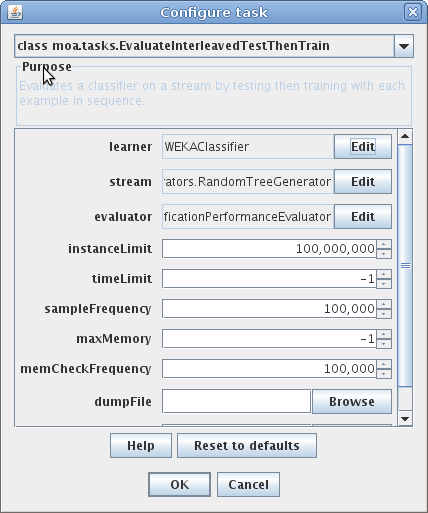
\includegraphics[height=5.5cm]{images/Screenshot-moa2.png}
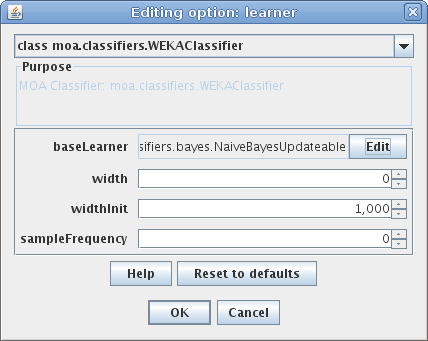
\includegraphics[height=2.5cm]{images/Screenshot-moa1.png}
\end{center}

To use the Weka classifiers from MOA it is necessary to use one of the following classes:

\subsection{WekaClassifier} A classifier to use classifiers from WEKA.

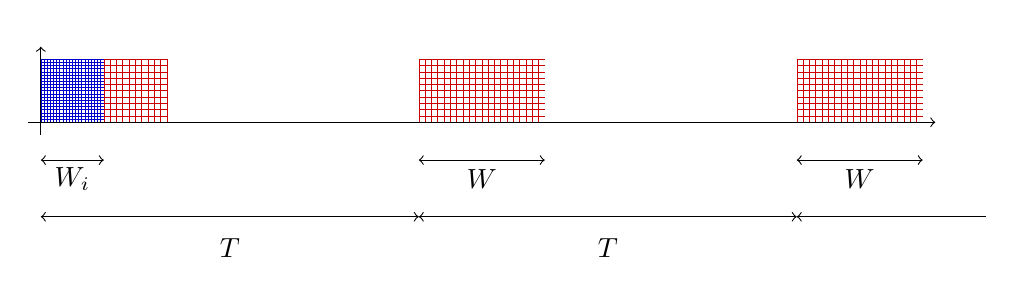
\begin{tikzpicture}[scale=.8,domain=0:18]
  \draw[step=.05,very thin,color=blue!80!black] (0,0) grid (1,1);
  \draw[step=.1 ,very thin,color=red!80!black] (1,0) grid (2,1);
  \draw[step=.1,very thin,color=red!80!black] (6,0) grid (8,1);
  \draw[step=.1,very thin,color=red!80!black] (12,0) grid (14,1);
  \draw[->] (-0.2,0) -- (14.2,0) node[right] {};
  \draw[->] (0,-0.2) -- (0,1.2) node[above] {};
  \draw[<->] (0,-0.6) -- (1,-0.6) node[below] {};
  \draw[<->] (6,-0.6) -- (8,-0.6) node[below] {};
  \draw[<->] (12,-0.6) -- (14,-0.6) node[below] {};
  \draw[<->] (0,-1.5) -- (6,-1.5) node[below] {};
  \draw[<->] (6,-1.5) -- (12,-1.5) node[below] {};
 \draw[<-] (12,-1.5) -- (15,-1.5) node[below] {};

  \draw (3,-2) node[] {$T$};
  \draw (9,-2) node[] {$T$};
  \draw (.5,-0.9) node[] {$W_i$};
  \draw (7,-0.9) node[] {$W$};
  \draw (13,-0.9) node[] {$W$};

\end{tikzpicture}

WEKAClassifier builds a model of $W$ instances every $T$ instances only for non incremental methods.
For WEKA incremental methods the WEKA classifier is trained for every instance.

 Example:
\begin{footnotesize}
\begin{verbatim}               
   meta.WekaClassifier -l weka.classifiers.trees.J48  
            -w 10000 -i 1000 -f 100000
\end{verbatim} \end{footnotesize}

Parameters:

\begin{itemize}
\item -l : Classifier to train
\item -w : Size of Window for training learner
\item -i : Size of first Window for training learner
\item -f : How many instances between samples of the learning performance
\end{itemize}

 \subsection{SingleClassifierDrift} Class for handling concept drift datasets with a wrapper on a
 classifier.

The drift detection method (DDM) proposed by Gama et al. controls 
the number of errors produced by the learning model during prediction. 
It compares the statistics of two windows: the first one contains all the data, 
and the second one contains only the data from the beginning until the number of
errors increases. Their method doesn't store these windows in memory. It keeps 
only statistics and a window of recent errors.

They consider that the number of errors in a sample of examples is modeled by a binomial 
distribution. A significant increase in the error of the algorithm, suggests
that the class distribution is changing and, hence, the actual decision model is
supposed to be inappropriate. They check for a warning level and a drift level. Beyond
these levels, change of context is considered.

%\BEGINOMIT
The number of errors in a sample of $n$ examples is modeled by a binomial 
distribution. For each point $i$ in the sequence that is being sampled, the error
rate is the probability of misclassifying ($p_i$), with standard deviation given
by $s_i = \sqrt{p_i(1 - p_i)/i}$. 
A significant increase in the error of the algorithm, suggests
that the class distribution is changing and, hence, the actual decision model is
supposed to be inappropriate. Thus, they store the values of $p_i$ and $s_i$ when
$p_i+s_i$ reaches its minimum value during the process (obtaining $p_{pmin}$ and $s_{min}$).
And it checks when the following conditions trigger:
\begin{itemize}
\item $p_i + s_i \geq p_{min} + 2 \cdot s_{min}$ for the warning level. 
	Beyond this level, the examples are stored in anticipation of a possible
	change of context.
\item $p_i + s_i \geq p_{min} + 3 \cdot s_{min}$ for the drift level. Beyond this
	level, the model induced by the learning method is reset and a new model
	is learnt using the examples stored since the warning level triggered.
\end{itemize}
%\ENDOMIT

Baena-Garc\'{\i}a et al. proposed a new method EDDM in order to improve DDM. 
It is based on the estimated distribution of the distances between classification errors.
The window resize procedure is governed by the same heuristics.

See more details in:

\begin{itemize}
\bibitem[GMCR]{Gama}
J.~Gama, P.~Medas, G.~Castillo, and P.~Rodrigues.
\newblock Learning with drift detection.
\newblock In {\em SBIA Brazilian Symposium on Artificial Intelligence}, pages
  286--295, 2004.

\bibitem[BDF]{EDDM}
Manuel Baena-Garc\'{\i}a, Jos{\'e} del Campo-{\'A}vila, Ra\'ul Fidalgo, Albert
  Bifet, Ricard Gavald\'a, and Rafael Morales-Bueno.
\newblock Early drift detection method.
\newblock In {\em Fourth International Workshop on Knowledge Discovery from
  Data Streams}, 2006.\end{itemize}

Example:
\begin{footnotesize}\begin{verbatim}
drift.SingleClassifierDrift -d EDDM 
    -l weka.classifiers.bayes.NaiveBayesUpdateable
\end{verbatim}\end{footnotesize}

Parameters:
\begin{itemize}
\item -l : Classifier to train
\item -d : Drift detection method to use: DDM or EDDM
\end{itemize}

\section{MOA classifiers from WEKA}

You can use MOA classifiers quite easily as incremental classifiers within the
WEKA Explorer, Knowledge Flow interface or command-line interface, using the \texttt{weka.classifiers.meta.MOA} meta-classifier.
This meta-classifier is just a wrapper for MOA classifiers, translating the
WEKA method calls into MOA ones.

\begin{center}
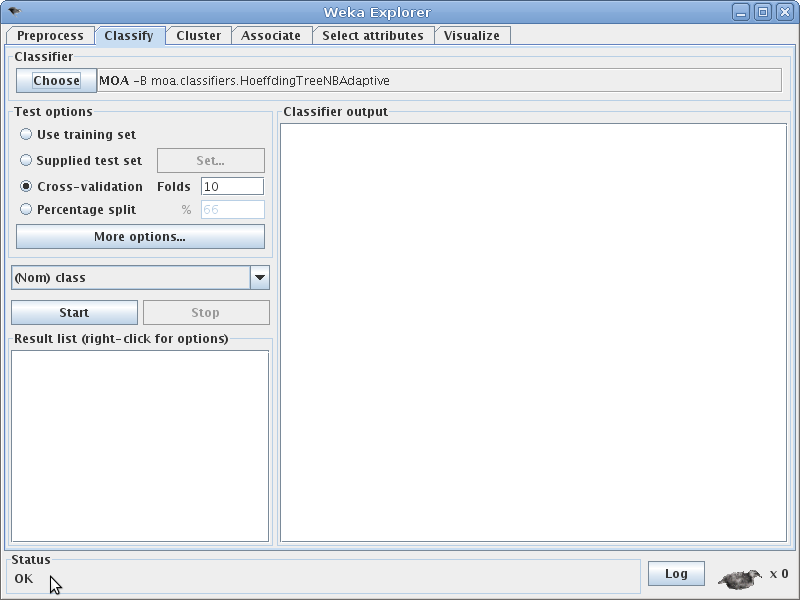
\includegraphics[height=5.5cm]{images/Screenshot-WekaE.png}
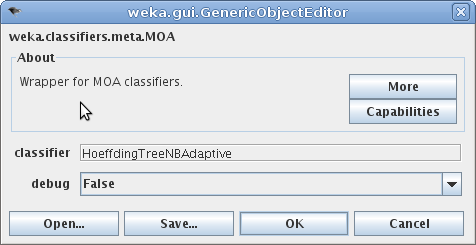
\includegraphics[height=2.5cm]{images/Screenshot-weka.png}
\end{center}

You can use MOA streams within the WEKA framework using the 

\texttt{weka.datagenerators.classifiers.classification.MOA}
\vspace{.2cm}

data generator.
For example:
\begin{footnotesize}\begin{verbatim}
  weka.datagenerators.classifiers.classification.MOA 
           -B moa.streams.generators.LEDGenerator
\end{verbatim}\end{footnotesize}

In order to manipulate the MOA classifiers in the GUI, like Explorer or
Experimenter, you need to register a new editor for the GenericObjectEditor.

The following steps are necessary to integrate the MOA classifiers:
\begin{enumerate}
 \item Determine the location of your home directory:
\begin{itemize}
 \item  Windows
     in a command prompt, run the following command:
       echo \%USERPROFILE\%
 \item Linux/Unix
     in a terminal (bash), run the following command:
       echo \$HOME
\end{itemize}
\item Copy the "GUIEdtitors.props.addon" file, contained in the MOA project in the 
   source directory "src/main/java/weka/gui" or in the moa.jar in "weka/gui",
   into your home directory. Rename the extension from ".props.addon" to 
   ".props". If the home directory already contains such a file, then just 
   append the content of the version in MOA file to the already existing one.

\item Restart WEKA from the MOA project, e.g., using the "run-explorer" target of
   the ANT build file.
\end{enumerate}   
\end{document}